\documentclass[11pt]{article}
\usepackage[paper1]{../paper_style/kirin-papers}
\usepackage[round,authoryear]{natbib}
\setcitestyle{aysep={,}}
\bibliographystyle{plainnat}

% Title block variant: this paper's repository instead of the looped-transformer one.
\renewcommand{\KirinTitleBlock}[7]{%
  \thispagestyle{fancy}%
  \begingroup
  \setlength{\parindent}{0pt}%
  \noindent\begin{minipage}[t]{0.72\linewidth}
    {\sffamily\bfseries\fontsize{8.5pt}{10pt}\selectfont\color{KirinAccent}\MakeUppercase{#1}}
  \end{minipage}%
  \begin{minipage}[t]{0.28\linewidth}
    \raggedleft{\sffamily\fontsize{8.5pt}{10pt}\selectfont\color{KirinMuted}#6}
  \end{minipage}\par
  \vspace{4pt}\color{KirinAccent}\hrule height 0.85pt\color{KirinInk}\vspace{9pt}
  {\sffamily\bfseries\fontsize{23pt}{25.2pt}\selectfont\raggedright #2\par}
  \vspace{4pt}
  {\sffamily\fontsize{15.2pt}{17.5pt}\selectfont\color{KirinAccentDark}\raggedright #3\par}
  \vspace{8pt}\color{KirinRule}\hrule height 0.45pt\color{KirinInk}\vspace{7pt}
  {\sffamily\bfseries\fontsize{11.5pt}{13.2pt}\selectfont #4}\par
  \vspace{2pt}
  {\sffamily\fontsize{8.9pt}{10.6pt}\selectfont\color{KirinMuted}%
    \href{https://github.com/VykosMolt}{github.com/VykosMolt}%
    \enspace\textcolor{KirinRule}{|}\enspace
    \href{https://github.com/VykosMolt/One-Concept-Multiple-Geometries}{github.com/VykosMolt/One-Concept-Multiple-Geometries}%
    \ifstrempty{#5}{}{\enspace\textcolor{KirinRule}{|}\enspace #5}%
  }\par
  \ifstrempty{#7}{}{\vspace{5pt}{\sffamily\fontsize{8.5pt}{10.2pt}\selectfont\color{KirinMuted}#7\par}}
  \vspace{6pt}
  \endgroup
}

\newcommand{\fl}{$\flat$}
\newcommand{\sh}{$\sharp$}
\newcommand{\Cb}{C\fl}\newcommand{\Gb}{G\fl}\newcommand{\Db}{D\fl}\newcommand{\Fs}{F\sh}\newcommand{\Cs}{C\sh}
\newcommand{\lc}{line$\,|\,$circle}
\newcommand{\cl}{circle$\,|\,$line}
\newcommand{\KL}{\mathrm{KL}}
\newcommand{\hd}[1]{{\sffamily\bfseries #1}}

\titleformat{\section}
  {\sffamily\bfseries\color{KirinAccent}\fontsize{15.2pt}{17.5pt}\selectfont}
  {\thesection}{0.6em}{}
\titleformat{\subsection}
  {\sffamily\bfseries\color{KirinInk}\fontsize{12.2pt}{14.2pt}\selectfont}
  {\thesubsection}{0.6em}{}
\KirinSetShortTitle{One Concept, Multiple Geometries}
\hypersetup{pdftitle={One Concept, Multiple Geometries: Corpus Operators Recover Different Structures, and Task-aligned Conditionals Predict Held-out Model Behaviour},pdfauthor={Jan Kirin}}

\begin{document}
\KirinTitleBlock
  {Research paper}
  {One Concept, Multiple Geometries}
  {Corpus operators recover different structures, and task-aligned conditionals predict held-out model behaviour --- with musical keys as the instrument}
  {Jan Kirin}
  {\href{https://orcid.org/0009-0005-2681-9027}{ORCID 0009-0005-2681-9027}}
  {August 2026}
  {Preprint. Every number in this paper traces to a results file in the repository; the chronological research log records which analyses were fixed before data were seen and which were added afterwards; \texttt{MANUSCRIPT\_AUDIT.md} records the hardening pass.}

\begin{abstractbox}
Representation-geometry studies often treat the geometry of a concept family as a property of the domain. We argue, on a natural domain, that the recovered geometry can depend on the statistical operator and on the task one measures. Musical keys are the instrument: neutral pitch classes close into the circle of fifths, on which enharmonic spellings such as C\fl{} and B coincide; tonal pitch classes lie on an open line of fifths, twelve steps apart \citep{temperley2000line,moss2023line}.

Symmetric co-occurrence statistics of English Wikipedia recover a robust periodic fifths structure (partial Spearman with fifths distance $+0.62$/$+0.66$, relabeling $p\le5\times10^{-4}$), and a naive Fourier analysis of the key-name activations of four language models appears to agree. That neural harmonic is an orthographic alias: a binary ``carries an accidental'' feature places 79.6\% of its Fourier energy in the fifths pair (31\% of all binary partitions of the twelve-cycle put half or more of their energy into one paired mode), a respelling intervention moves the block with the glyph, and only the 7B model keeps a controlled fifths signal.

The models' next-key behaviour --- sequence probabilities over a fixed candidate set of key-name continuations, row-normalized --- instead follows the open line in all four models. An ordered key-mention conditional $p(j\mid i)$ from a 40-word window aligns with those distributions far better (Spearman $\approx0.80$) than PMI-type association operators built from the same or from Karkada-style counts ($0.1$--$0.5$); directionality itself contributes nothing, a symmetrized conditional from the same counts doing equally well. Beyond circle, line, orthography and frequency baselines --- and beyond a training-row target prior --- the corpus conditionals reduce the held-out KL of next-key distributions by 14--34\% (6--28\% under a rich theory model; $b=0$ of $5{,}000$ relabelings in the flagship cells). The gain replicates across corpora; corpus specificity is inconclusive. Synthetic controls show that output-code geometry and sparse-alias learning are insufficient for the converged line. In this domain, the geometry one recovers depends on the operator, the equivalence relation and the task that define it.
\end{abstractbox}

\par\vspace{4pt}
\noindent\begin{minipage}{\linewidth}
\centering
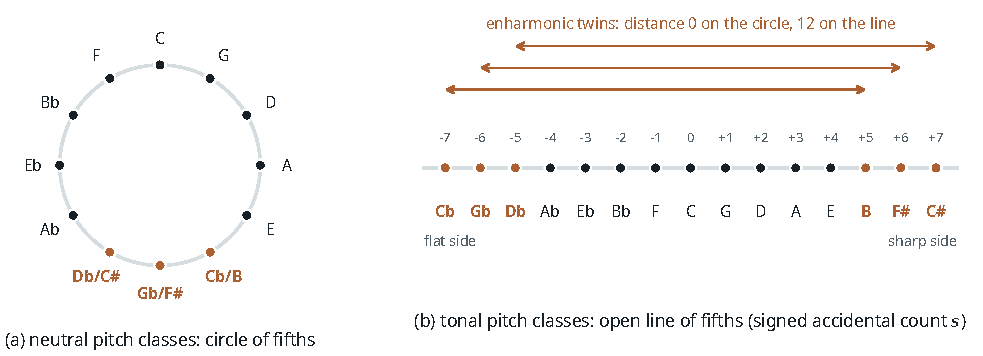
\includegraphics[width=.96\linewidth,keepaspectratio]{figures/fig_spaces.pdf}
\kirinfigcaption{Figure 1.}{The two tonal spaces used throughout. (a) Neutral pitch classes identify enharmonic spellings and close into the circle of fifths. (b) Tonal pitch classes keep spellings distinct on an open line indexed by the signed accidental count $s$ of the key signature ($-7$ = seven flats, $+7$ = seven sharps); the three standard enharmonic pairs (orange) are distance 0 on the circle and 12 on the line. Over the 105 pairs of the 15 standard major-key spellings the two distance matrices correlate only $\rho=0.25$ (vs.\ $0.68$ for the conventional 12-key set), which is what makes the 15-key design discriminative.}
\end{minipage}

\section*{Results at a glance}\label{sec:glance}

\begin{glancebox}
\noindent\textbf{Question.} Is there a single ``geometry of musical keys'' to be read off language statistics or language-model activations --- and if the answer differs across measurements, which measurement predicts what?

\smallskip\noindent\textbf{What is established.} (``$X\,|\,Y$'' denotes the partial Spearman correlation of a distance matrix with geometry $X$ controlling for geometry $Y$ and for orthographic and commonness features, \S\ref{sec:setup}; ECI is the enharmonic collapse index defined in \S\ref{sec:corpus}.)
\begin{itemize}
\item \emph{Symmetric corpus statistics are periodic.} Wikipedia PMI over the 12 major keys decreases with circular fifths distance (partial $+0.62$ canonical / $+0.66$ enharmonic-merged, $p\le5\times10^{-4}$ under two null families); with enharmonics merged, \cl{} $=+0.58$ [shard-cluster 95\% CI $+0.39, +0.64$], \lc{} $=-0.07$ [$-0.20, +0.07$] (\S\ref{sec:corpus}).
\item \emph{Naive representation instruments are fooled by orthography.} The fifths Fourier pair of key-name activations is dominated by an accidental-glyph indicator that carries 79.6\% of its energy in that pair; respelling white keys moves the block with the glyph; after controls only OLMo-2-7B keeps a layer-corrected fifths partial ($p=.046/.018$, 1,000 relabelings) (\S\ref{sec:alias}).
\item \emph{Behaviour follows the open line.} Restricted next-key distributions (sequence probability over a fixed candidate set, row-normalized) of all four models are ordered by the signed accidental count (\lc{} $+0.27$…$+0.56$, 4/4 templates significant under glyph-preserving nulls in 14 of 16 model$\times$family cells); the line survives enharmonic-merged scoring at roughly two thirds strength (\S\ref{sec:behaviour}).
\item \emph{Conditional-row operators align with behaviour far better than association operators; directionality per se contributes nothing.} Spearman with next-key behaviour (1B/Gemma/Qwen/7B): window conditional $+0.80/{+}0.78/{+}0.79/{+}0.80$, a symmetrized conditional from the same counts $+0.82/{+}0.78/{+}0.80/{+}0.81$, helper-word factorization $+0.68/{+}0.67/{+}0.64/{+}0.65$, Karkada-window PMI $+0.39/{+}0.46/{+}0.40/{+}0.54$, a PMI from the same 40-word counts $+0.12/{+}0.16/{+}0.10/{+}0.24$ (\S\ref{sec:operators}).
\item \emph{Corpus conditionals add held-out predictive value beyond theory geometry and beyond a training-row target prior.} Target-aggregated modulation family: $\Delta\KL=+0.037/{+}0.029/{+}0.016/{+}0.036$ nats per row against a theory KL of $0.12$--$0.13$ (relabeling $p\le8\times10^{-4}$, $B=5{,}000$; document-cluster bootstrap intervals exclude zero); $+0.023/{+}0.019/{+}0.007/{+}0.018$ with quadratic and harmonic theory terms ($p\le.013$); $+0.041/{+}0.035/{+}0.025/{+}0.047$ with a training-row target prior in the baseline; within-row $\Delta R^2$ $0.19$--$0.38$ (\S\ref{sec:heldout}).
\item \emph{Generic across corpora; specificity inconclusive.} Every corpus, including 633- and 3,843-pair DCLM samples, gives the gain in every model. The OLMo-vs-others difference-in-differences against size-matched Wikipedia reaches $p<.05$ in 10 of 72 pre-registered cells, all positive but small ($0.004$--$0.05$ nats), six separating both OLMo models from both others and four carried by the 7B alone; in the target-aggregated view it is $\approx0$ in the modulation family on every DCLM sample (\S\ref{sec:cross}).
\item \emph{Two artifact explanations are excluded by causal test.} A line-aligned output code over a perfectly periodic law leaves converged behaviour periodic (KL to oracle $\le0.001$; twin asymmetry $+0.013$) while tilting the predictive-state representation by $+0.08$…$+0.10$ (5/5 seeds); sparse aliases converge as a power law in exposures and an equally rare unique state is learned just as well (\S\ref{sec:synthetic}).
\item \emph{Acquisition order (one run).} Along OLMo-2-1B checkpoints \lc{} rises from $-0.24$ (1B tokens) to $+0.19$ (21B) and $+0.33$ (4T); the residual correspondence is first significant at 294B tokens ($p=.037$) and stable from 4T ($p\le.017$); stage-2 training raises the line in 3/3 seeds ($+0.09$…$+0.11$) but not the residual ($+0.01$…$+0.04$) (\S\ref{sec:trajectory}).
\end{itemize}

\smallskip\noindent\textbf{What is not claimed.} That LLMs ``contain'' or ``reason with'' a circle of fifths; a circle-to-line transition across layers; a privileged predicting-position locus; a scaling trend; separable circle/line/spelling subspaces; a tokenization or rare-alias explanation of the line; or that behaviour fingerprints a model's training corpus (nor that it does not). Each of these was proposed during the project and killed by a control, a null or an independent review (Appendix~A).
\end{glancebox}

\begin{roadmapbox}
\S\ref{sec:intro} motivates the question and places it in the literature. \S\ref{sec:setup} fixes the objects: the 12- and 15-key designs, models, corpus, extraction families and nulls. \S\ref{sec:corpus}--\S\ref{sec:alias} treat the symmetric statistic and the instrument failure. \S\ref{sec:behaviour}--\S\ref{sec:cross} contain the main result: behaviour, operators, held-out prediction, corpus genericity. \S\ref{sec:synthetic} presents the two synthetic falsification experiments compactly; \S\ref{sec:trajectory} the checkpoint series. \S\ref{sec:discussion} states the synthesis and limitations. The repository is organized in five sequential phases (I: 12-key corpus and geometry; II: 15-key design; III--IV: synthetic controls; V: conditionals, cross-corpus and checkpoints); where the text names a phase it identifies which log and design document fixed the analysis. Appendix~A lists every retracted claim and post-hoc decision; Appendix~B gives the Fourier bookkeeping; Appendix~C the full tables; Appendix~D the methods in full.
\end{roadmapbox}

\section{Introduction}\label{sec:intro}

A growing body of work reads geometric structure off the internal representations of language models --- circles for weekdays and months \citep{engels2025not}, lines and helices for numbers \citep{gurnee2024space,bassi2026ordinal}, lattices for grids \citep{brenner2026grid} --- and explains it from the statistics of the training text. \citet{karkada2026symmetry} give the sharpest version of that explanation: when a word-word association statistic is translation-symmetric over a concept family, word2vec-like models embed the family on a Fourier lattice whose harmonic amplitudes are set by the statistic's spectrum, and residual streams of transformers show the same qualitative picture. A different tradition \citep{zhao2024implicit,zhao2025geometry} derives geometry from the \emph{directional} object that next-token prediction actually optimizes: the conditional distribution of the next token given the context and its support pattern.

These are different operators over the same text. For most concept families that have been studied they happen to agree on the answer, because the family has one obvious ordering. Musical keys do not. Twelve pitch classes carry two competing cyclic orderings, chromatic ($x\mapsto x+1$) and fifths ($x\mapsto x+7$), related by an automorphism of $\mathbb{Z}_{12}$; and, more importantly, music theory itself distinguishes two spaces for the same keys. In the \emph{neutral} pitch-class space of pitch-class set theory, enharmonic spellings (C\fl{} and B) are the same object and the keys close into the circle of fifths. In the \emph{tonal} pitch-class space of \citet{temperley2000line} and \citet{moss2023line}, spellings are retained, keys live on an open line of fifths indexed by key-signature accidentals, and C\fl{} major sits twelve steps from B major (Figure~1). Neither space is ``more correct''; they are different equivalence relations, and --- the burden of \citet{moss2023line}'s point that neutral (MIDI-like) encodings discard the distinction --- the representation format of the data decides which of the two can be recovered at all.

This paper uses that fact as an instrument. We ask which geometry appears under which corpus operator and which model measurement, and --- the quantitative core --- which operator predicts held-out model behaviour after the obvious geometric and orthographic explanations are removed. The project began as a cheap test of the symmetric statistics-to-geometry theory on a family with competing orderings, and its first result was a convincing false positive: the fifths harmonic in key-name activations turned out to be an orthographic feature. What survived several rounds of controls and two synthetic attempts to explain the natural result away is a different and, we think, more general claim:

\begin{scopebox}[{Central claim}]
Different statistical operators over the same concept family expose different, independently legitimate geometries. For keys, PMI-type association statistics identify the enharmonic spellings and carry robust periodic fifths structure; conditional-row operators built from the same local counts separate the spellings that association identifies, whether the conditional is directional or symmetrized, while remaining fifths-smooth. Model behaviour --- restricted next-key distributions over a fixed candidate set --- lies on the spelling-sensitive open line, and it is the local conditional operators, not the association operators tested, that align with it and add held-out predictive value beyond explicit circle, line, orthography and frequency baselines --- generically across models and corpora; whether any part of it is specific to a model's own training data is left open (\S\ref{sec:cross}).
\end{scopebox}

\paragraph{Contributions}
(1)~\emph{Operator-dependent tonal geometry}: association and conditional-row statistics over one natural concept family recover distinct structures that map onto the neutral/tonal pitch-class distinction, and a matched control shows the contrast is one of construction, not of directionality (\S\ref{sec:corpus}, \S\ref{sec:operators}).
(2)~\emph{Conditional corpus statistics predict restricted next-key behaviour}: across four models, local key-mention conditionals improve held-out prediction of next-key distributions beyond explicit geometric, orthographic and frequency baselines, with permutation nulls and a rich-theory robustness check (\S\ref{sec:heldout}); the gain is generic across corpora, and a test of corpus specificity is inconclusive (\S\ref{sec:cross}).
(3)~\emph{A concrete failure mode of Fourier representation analysis}: a categorical orthographic feature contiguous on the chosen cyclic ordering produces dominant, semantic-looking harmonics; a respelling intervention exposes it (\S\ref{sec:alias}).
(4)~\emph{Artifact explanations tested causally}: controlled synthetic experiments bound what output-code structure and sparse alias exposure can do (\S\ref{sec:synthetic}).
(5)~\emph{Suggestive acquisition evidence}: one checkpointed pretraining run shows coarse tonal structure earlier than the finer residual correspondence with corpus conditionals (\S\ref{sec:trajectory}).

\paragraph{What is not new} Circle-of-fifths geometry in models trained on \emph{music} is established \citep{chuan2020context,huang2016chordripple,sadek2026circle}; the line of fifths as tonal structure goes back to Weber's 1821 spiral, straightened by \citet{temperley2000line}; the coexistence of string and semantic geometry \citep{marjieh2025number}, context-dependent concept geometry \citep{hu2026shared}, transient mid-layer perceptual geometry \citep{singh2026geometry}, correlation-driven feature geometry \citep{prieto2026data}, factored representations \citep{shai2026factored}, and the correspondence of activation geometry with behaviour \citep{wurgaft2026manifold} are all known; the DFT of the diatonic/black-key set peaking at the fifth coefficient is textbook in mathematical music theory \citep{quinn2006general,amiot2016music}; a Fourier-looking representation need not imply a Fourier algorithm \citep{nanda2023progress,zhong2023clock,feucht2026arithmetic}; and Fourier sparsity is necessary but not sufficient for linear separability \citep{fu2026convergent}. The conjunction --- a natural family with two motivated geometries, operator-dependent recovery, held-out behavioural prediction by the task-aligned operator, and a realistic demonstration of the orthographic false positive --- is what we claim.

\section{Setting}\label{sec:setup}

\subsection{Keys, coordinates and geometries}
Pitch classes are indexed by semitone $x\in\mathbb{Z}_{12}$ (C $=0$). Since $7^2\equiv1 \pmod{12}$, $r(x)=7x \bmod 12$ is an involutive automorphism that maps ascending fifths to unit steps; a fifths-smooth kernel is circulant in semitone coordinates, so \emph{circulant structure alone cannot distinguish the chromatic from the fifths ordering} --- only the Fourier index can. For centered representations $h_x$ of the twelve concepts, $\hat h_k = 12^{-1/2}\sum_x h_x e^{-2\pi i kx/12}$, $E_k=\|\hat h_k\|^2$, and we report the paired energies $P_m=E_m+E_{12-m}$ ($m=1,\dots,5$) and $E_6$. Under $x\mapsto7x$ only $P_1$ and $P_5$ exchange; $P_2,P_3,P_4,E_6$ are invariant (verified numerically, Appendix~B). $P_1$ is the chromatic fundamental, $P_5$ the fifths fundamental. Simultaneous $P_1$ and $P_5$ energy is one 12-point orbit with two harmonics, not a torus (the Krumhansl--Kessler key torus is a different, two-variable object over 24 keys; \citealp{krumhansl1982tracing}).

The \textbf{12-key design} uses the conventional spellings C, D\fl, D, E\fl, E, F, F\sh, G, A\fl, A, B\fl, B. The \textbf{15-key design} uses the fifteen standard major-key spellings on the signed line $s=-7$ (C\fl) $\ldots$ $+7$ (C\sh), so that (C\fl, B), (G\fl, F\sh), (D\fl, C\sh) share a neutral pitch class: circle distance 0, line distance 12. Candidate geometries over the 105 pairs: circle of fifths, line of fifths, chromatic, the orthographic family (glyph class, has-accidental, edit distance, root-letter identity, alphabet distance, token count) and log commonness. The classical tonal spaces add no discrimination on major keys alone --- Krumhansl--Kessler major--major similarity is $\rho=0.99$ with the circle and Chew's spiral array \citep{chew2000towards} $\rho=1.00$ with the line --- so we report circle vs line and leave them for a minor-key extension. Unless stated otherwise, corpus kernel and key-name geometry statistics use the 12-key design (66 pairs) and behavioural, operator and held-out statistics use the 15-key design (105 pairs).

\subsection{Models, corpus and behavioural task}
Models: OLMo-2-0425-1B, Gemma-2-2B, Qwen2.5-3B and OLMo-2-1124-7B, base checkpoints \citep{olmo2,gemma2,qwen25}; forward passes only, on one 12\,GB laptop GPU. Slash-separated lists of four numbers follow this order (OLMo-1B / Gemma / Qwen / OLMo-7B) unless stated otherwise. Corpus: English Wikipedia 20231101 (41 shards, 6.41M documents, $\approx3.1$B words), the dump used by \citet{karkada2026symmetry}, scanned with their window ($L=16$, $f(d)=17-d$) for symmetric statistics and with the directional extraction families of \S\ref{sec:operators} for conditionals. Behaviour: six context families were written for the 15-key design (A spelling, B enharmonic equivalence, C harmonic relation, D chord progression, E modulation/next key, F generic mention), four templates each; key-name geometry statistics (\S\ref{sec:alias}) use all six, behavioural matrices the four relational families B--E, and the held-out tests of \S\ref{sec:heldout} families C, D and E. For each source key $i$ and family, the sequence log-probability of every candidate continuation ``\,$j$ major'' over the 15 spellings, row-normalized over the candidate set --- a $15\times15$ matrix $Q$. This is restricted-candidate behaviour, not free generation: the model is never asked to produce text, only to assign probability to fifteen complete continuations (Appendix~D). Three behavioural scorers were pre-registered: the \emph{total} sequence log-probability (primary), the \emph{length-normalized} scorer (per-token mean), and the \emph{enharmonic-merged behavioural scorer}, which pools the two spellings of each twin before scoring and therefore applies only to families whose task is neutral to spelling (B, C, D). Distinct from all three is the \emph{12-class target-aggregated view} of \S\ref{sec:heldout}, a diagnostic projection of the already-scored candidate distribution onto 12 pitch classes; we report the \emph{spelled} view (15 targets) and this \emph{target-aggregated} view side by side, neither privileged.

\subsection{Statistics and nulls}
Geometry is compared by representational similarity analysis (RSA: Spearman correlation over pairs of distances) and by partial Spearman correlations \lc{} and \cl{}, each controlling for the other and for the orthographic and commonness features. Every partial carries a relabeling null (free, and glyph-class-preserving where an orthographic block is a plausible nuisance); best-over-layers values carry a max-over-layers null that repeats the selection; context contrasts use template-regrouping nulls on an a-priori layer band; corpus statistics carry a shard-cluster bootstrap, the flagship held-out gain a document-cluster bootstrap. With 12--15 concepts the pairwise observations are not independent, and we never quote asymptotic $p$-values.

\section{Symmetric corpus statistics recover a periodic fifths structure}\label{sec:corpus}

Months are the positive control: the Karkada statistic $M^*$ over Wikipedia is 97\% circulant with paired spectrum $0.50$, $0.26$, $0.12$, $0.08$, $0.03$, $0.01$ ($P_1$…$P_5$, $E_6$), converged by 0.1B words, and OLMo-2-1B's month-name Fourier profile matches it (best-layer cosine $0.97$--$0.99$, per-layer minima $0.82$--$0.94$; a flat null profile gives $0.75$).

For keys $M^*$ saturates: $P_{ij}\gg P_iP_j$ drives every off-diagonal entry to $1.97$--$2.00$ and the $12\times12$ ``spectrum'' is numerical residue that flips with corpus size --- a finding about the statistic itself on a dense block of rare tokens, not a caveat about comparability. We therefore use PMI, to which skip-gram with negative sampling is related through the factorization of shifted PMI \citep{levy2014neural}; the two agree at full-vocabulary level (RSA $+0.43$ vs $+0.44$) but the $12\times12$ comparisons are PMI-only, and PMI and $M^*$ are not interchangeable. The PMI kernel in fifths order is $8.64, 7.89, 7.59, 7.16, 7.07, 7.13, 6.48$ for $d'=0,\dots,6$ --- decreasing with fifths distance (one wobble at $d'=5$), jagged in semitone order (Figure~2b). The naive Fourier share $P_5=0.50$ vs $P_1=0.17$ depends on the PMI diagonal $\kappa(0)$ (removing it inverts the profile), so the robust statement is the kernel, not the spectrum.

\par\vspace{4pt}
\noindent\begin{minipage}{\linewidth}
\centering
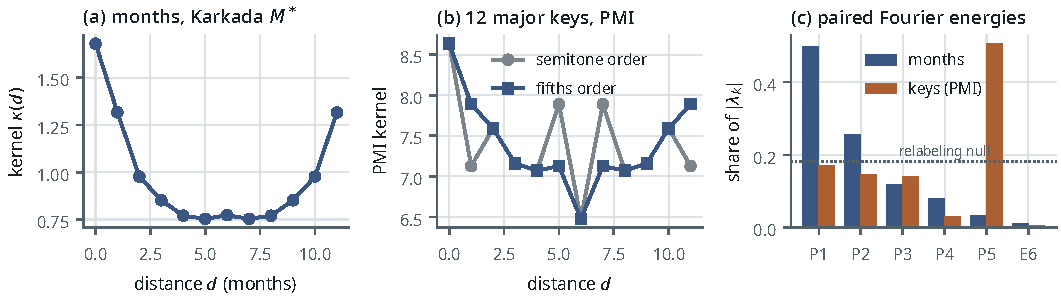
\includegraphics[width=.96\linewidth,keepaspectratio]{figures/fig_corpus.pdf}
\kirinfigcaption{Figure 2.}{Symmetric corpus statistics. (a) The months kernel (positive control). (b) The keys PMI kernel is jagged in semitone order and smooth in fifths order. (c) Paired Fourier shares of $|\lambda_k|$ (months from $M^*$, keys from PMI; $M^*$ is saturated for keys and its key spectrum is not shown); the keys' $P_5$ share is diagonal-dependent and is not the evidence --- the controlled partials are.}
\end{minipage}

\begin{resultbox}[{Result 1 --- the corpus fifths structure is real, ordering-specific and periodic}]
Partial Spearman of PMI with fifths distance, controlling for the accidental block, log commonness, letter identity and alphabet distance: $+0.62$ (canonical spellings), $+0.66$ (enharmonics merged), $p\le0.0005$ (the resolution of the 2000-relabeling null) under both the free and the block-preserving relabeling null. The white-key sub-block ordered F--C--G--D--A--E--B ranks 78th of 5040 orderings ($p=0.016$). Removing every document that mentions ``circle of fifths'' or ``perfect fifth'' changes nothing ($+0.64$). A Karkada-style helper-word factorization applied to the PMI matrix --- $W=\Phi\sqrt{|\Lambda|}$ of the $V=3000$ PMI over the 14,235 key-containing documents --- reproduces the key rows' fifths partial at $+0.52$…$+0.56$, unchanged when the $12\times12$ key block is zeroed before factorizing (the block is $\approx1\%$ of the matrix, so this ablation is close to tautological): helper vocabulary carries the structure, as in their Fig.~4. Topology (12-key, 66 pairs): circle vs line, each controlling for the other, gives \cl{} $=+0.40$ and \lc{} $=+0.27$ in the canonical family and \cl{} $=+0.58$, \lc{} $=-0.07$ with enharmonics merged. Uncertainty from a shard-cluster bootstrap (the 41 Wikipedia shards resampled with replacement, which preserves within-document dependence; 1,000 resamples): fifths partial $+0.62$ [95\% CI $+0.44$, $+0.68$] canonical and $+0.66$ [$+0.49$, $+0.71$] merged; merged \cl{} $+0.58$ [$+0.39$, $+0.64$] and \lc{} $-0.07$ [$-0.20$, $+0.07$], with $P(\cl>\lc)=1.00$; canonical \cl{} $+0.40$ [$+0.05$, $+0.55$] and \lc{} $+0.27$ [$-0.08$, $+0.58$], $P=0.63$ --- the canonical set starves the seam pairs because Wikipedia is spelling-consistent per document (D\fl$|$F\sh{} weighted count 17 vs D\fl$|$G\fl{} 160), so we lead with the merged family. (An earlier Poisson-on-counts bootstrap gave $\pm0.02$/$\pm0.03$ and $P=0.87$ for the canonical family; it ignores document clustering and is withdrawn.)
\end{resultbox}

Over the 15 spellings (105 pairs) the symmetric statistic is both periodic and open: the three enharmonic pairs are the closest pairs of all --- the enharmonic collapse index (ECI), the mean percentile rank of the three twin distances among all pairs ($0$ = closest of all, $0.5$ = null), is $0.04$ (shard-cluster bootstrap 95\% CI $[0.03, 0.44]$: the upper tail reflects the 38 mentions of C\fl{} major); PMI $9.9$--$11.0$ vs median $7.3$ --- while \cl{} $=+0.42$ and \lc{} $=+0.38$ ($p\le.001$: $b=0$ of $1{,}000$ under both the free and the glyph-preserving null). A document scan finds only 41 co-mentions of enharmonic pairs in all of Wikipedia, half of them containing the word ``enharmonic'' and most of the rest slash notation: the corpus's neutral-pitch identity at the seam is metalinguistic, not harmonic usage. Cue-conditioned symmetric statistics (pairs split by intervening chord, key-signature, modulation or enharmonic cues) are circle-dominant in every class, including key-signature prose ($+0.68/0.00$).

\section{Naive key-name geometry is an orthographic alias}\label{sec:alias}

Key-name activations of the four models (24 contexts $\times$ 12 keys $\times$ all layers, three token positions) show a fifths Fourier share $P_5$ of $0.26$--$0.55$ with $P_1$ at the null --- in every template, position and spelling variant. This is what the months instrument, applied verbatim, reports; the first draft of this project called it a circle of fifths.

\begin{resultbox}[{Result 2 --- the fifths harmonic is an accidental-glyph feature}]
The five conventionally spelled keys with an accidental (D\fl, E\fl, F\sh, A\fl, B\fl) are contiguous on the circle of fifths, so a binary ``has an accidental'' indicator is a width-5 boxcar in fifths coordinates and places 79.6\% of its Fourier energy in the $k=5/7$ pair under the semitone labelling (exact; Figure~3a). Projecting this indicator out drops the models' $P_5$ to $0.11$--$0.14$, \emph{at} the projection-matched relabeling null of $0.12$ ($z\approx+0.4$); the $k=7$ mode is rank-1-like (isotropy $0.4$--$0.65$ vs $0.98$ for a circle); a synthetic calibration reproduces the observed numbers with boxcar-plus-noise and excludes a $\ge50\%$ genuine circle admixture. The component follows accidental-glyph/spelling structure rather than black-key membership: respelling four \emph{white} keys as B\sh, F\fl, E\sh, C\fl{} makes ``carries an accidental glyph'' (9 of 12) differ from ``is a black key'' (5 of 12), and the Gram RSA with the black-key block falls from $+0.70$…$+0.86$ to $-0.14$…$+0.12$ in all four models while the RSA with the glyph block rises to $+0.5/{+}0.4/{+}0.7/{+}0.3$ (OLMo-1B/Gemma/Qwen/OLMo-7B; Figure~3b). The failure mode is not peculiar to this feature: of the 4,094 nontrivial binary partitions of the 12-cycle, 24.7\% put more than half their centered Fourier energy into a single paired mode and 31.4\% put half or more --- a categorical attribute mimicking a cyclic fundamental is the common case, not the exception (Appendix~B).
\end{resultbox}

\par\vspace{4pt}
\noindent\begin{minipage}{\linewidth}
\centering
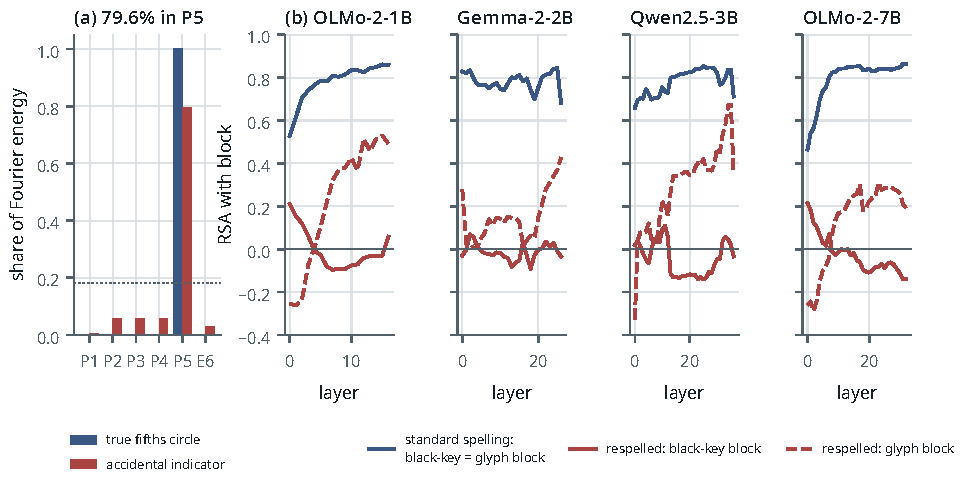
\includegraphics[width=.96\linewidth,keepaspectratio]{figures/fig_alias.pdf}
\kirinfigcaption{Figure 3.}{The false neural circle. (a) Paired Fourier shares of a true fifths circle and of the binary accidental indicator: the indicator alone is a convincing ``$P_5$ signal''. (b) Respelling intervention, per layer: with standard spellings the black-key and accidental-glyph blocks coincide (blue); after respelling C, E, F, B as B\sh, F\fl, E\sh, C\fl{} the block follows the glyph (dashed red), not the black keys (solid red). The respelled strings are rare, so glyph and rarity remain entangled; key-signature membership is ruled out.}
\end{minipage}

What remains after controls is small. With the glyph block, commonness, letter identity and alphabet distance partialled out, the best-layer fifths partials are $+0.21/{+}0.29/{+}0.23/{+}0.34$ (OLMo-1B/Gemma/Qwen/7B); with max-over-layers correction only the 7B model is significant ($p=0.046$ free / $0.018$ block-preserving; 1,000 relabelings, $(b+1)/(B+1)$), the other three are at $p=0.09$--$0.25$. The apparent scale curve is three noise-level points and one significant one. Even the 7B signal is line-like (\cl{} $\approx0$, \lc{} $+0.2$…$+0.3$), not an isotropic circle, and is lost at the final layer. Phase-II analyses with the 15-key design add two more instrument facts. First, the \emph{last token} of a multi-token key name is the accidental token for two-token keys and the letter token otherwise; probing it produced a line in the key-name geometry of Qwen and 7B ($+0.26$…$+0.37$, significant in all six context families) that disappears entirely under a span-mean probe (\lc{} $\approx0$ everywhere) --- there is no neutral key-token probe when concept names tokenize differently, and only the shared prompt-final position is token-uniform. Second, the general aliasing fact: a contiguous block of width $w=1,\dots,6$ on the 12-cycle puts $18/37/55/70/80/83\%$ of its energy in the fundamental pair; of all 4094 nontrivial binary partitions, a quarter (24.7\%) put more than half their centered energy in a single paired mode and 6.6\% more than 70\% (a further 6.7\% sit exactly at one half, so 31\% reach half or more); root-letter identity itself puts 34\% in the chromatic pair. \emph{Fourier power measures variation with respect to a chosen labelling; it does not identify the feature that caused it.} \citet{karkada2026symmetry}'s Appendix~D notes that cyclic and binary attributes can coexist in different spectral sectors; the point here is that a binary attribute can land in the cyclic sector.

At the token-uniform prompt-final position, cross-validated rank regressions show orthography and commonness explaining a cross-validated $R^2$ of $0.1$--$0.55$ of pair distances with circle or line adding $\le0.04$ in every cell; OLMo-2-7B has a periodic component at this position in all six context families, relational and non-relational alike (\cl{} $+0.21$…$+0.36$, $p=.006$--$.03$ with 500 relabelings and the $(b+1)/(B+1)$ estimator), so it is not a context effect; Gemma has an open one in some families; and cross-fitted ``spelling'' and ``semantic'' subspaces overlap heavily (held-out variance shares $0.53$--$0.73$ and $0.46$--$0.66$, summing above one): separable circle/line/spelling subspaces are not supported. Context effects on the periodic component are small ($+0.04$…$+0.07$ band-averaged, only Qwen at $p<.05$). Hidden-state geometry is therefore not where this paper's positive claim lives.

\section{Next-key behaviour follows the open line}\label{sec:behaviour}

\begin{resultbox}[{Result 3 --- the behavioural space is Temperley's line}]
With the 15-key design and the total scorer, \lc{} (the partial correlation of the behavioural distance matrix with line distance, controlling for circle distance, orthography and commonness) over 105 pairs is $+0.27$…$+0.44$ (OLMo-2-1B), $+0.32$…$+0.54$ (Gemma-2-2B), $+0.31$…$+0.52$ (Qwen2.5-3B) and $+0.14$…$+0.56$ (OLMo-2-7B) across the four context families, with all four templates significant under the glyph-preserving null in 14 of 16 model$\times$family cells; \cl{} is $\approx0$ ($-0.14$…$+0.11$) in the three smaller models and $+0.13$…$+0.28$ in the 7B. The first principal axis of the 12-key predictive matrices tracks the signed accidental count ($|\rho|=0.70$--$0.80$). Top-1 answers in the relational families are $\pm1$ line steps (dominant, subdominant). Merging the two spellings of each black key removes about a quarter to a third of the effect (Phase-I 12-key merged-\emph{target} scoring, modulation contexts: \lc{} $+0.69\to+0.46$, $+0.74\to+0.52$, $+0.79\to+0.66$, $+0.74\to+0.56$), and under the 15-key enharmonic-merged \emph{scorer} --- which by construction applies to the harmonic-relation, chord and enharmonic families, not to modulation --- \cl{} turns positive in every model ($+0.14$…$+0.52$): the empirical distinction between the two spaces is concentrated at the seam --- in enharmonic identification and boundary closure --- and once twins are pooled the periodic component reappears. Adding the model's own column marginal as a control \emph{raises} the predictive partials, so these values are conservative. \textbf{Scorer robustness.} Under the pre-registered length-normalized scorer the line survives in every cell: modulation \lc{} $+0.44\to+0.37$ (1B), $+0.54\to+0.43$ (Gemma), $+0.52\to+0.50$ (Qwen), $+0.56\to+0.45$ (7B), all 4/4 templates significant under the glyph-preserving null; over the 16 model$\times$family cells the count of significant templates drops from 63/64 to 58/64 (Table~C.6), \cl{} moves by at most $0.10$ and changes sign nowhere that matters, and twins move closer (ECI falls by $0.05$--$0.25$) without approaching identification.
\end{resultbox}

Enharmonic identity --- the defining property of the neutral space --- is known behaviourally by the 7B model only, with Qwen intermediate: asked for ``the enharmonic equivalent of X major'' it answers the twin (ECI $0.11$ total / $0.05$ length-normalized; top-1 interval $+12$ in 8--9 of 15 keys), Qwen partially ($0.51$), OLMo-1B ($0.70$) and Gemma ($0.83$) not at all; outside that family every model keeps twins far apart (ECI $0.67$--$0.90$). Few-shot fifth-relation accuracy is higher in the larger models (dominant $0.08/0.33/0.75/0.92$ under the raw scorer, a lower bound because it under-selects two-token names); with four models from four families this is not a scaling trend, and the geometric statements above show no such ordering.

So the corpus's symmetric statistic is periodic and the models' behaviour is open. Phase II concluded from the cue-conditioned symmetric statistics that ``the corpus contains no task-conditioned line''. That conclusion depended on a convention: it booked spelling class as an orthographic nuisance. Under \citet{temperley2000line} and \citet{moss2023line}, the signed accidental count of the key signature \emph{is} the tonal coordinate, and in text spelling class and that coordinate are the same variable. Which convention is right is a music-theoretic question the data cannot decide, and the next section replaces the question with one they can.

\section{Conditional-row operators align with behaviour far better than association operators}\label{sec:operators}

Instead of asking whether the corpus ``is'' a circle or a line, we ask which corpus operator predicts which model observable. Three operators are computed on the same Wikipedia text over the 15 spellings: (\emph{SYM}) the symmetric PMI of Karkada's $L=16$ distance-weighted window; (\emph{HELP}) the helper-word factorization $W=\Phi\sqrt{|\Lambda|}$; (\emph{COND}) the ordered key-mention conditional $p(j\mid i)$, rows of the $15\times15$ count matrix $N$ of mentions of key $j$ within 40 words after key $i$ (extraction family A; document-level and cue-conditioned variants B--D are defined in \S\ref{sec:heldout}), with row geometry given by Jensen--Shannon distances between rows. Because SYM and COND differ in several respects at once (symmetry, window, weighting, normalization, distance construction), three \emph{matched} operators are built from the same $N$: a symmetrized conditional (rows of $N+N^{\top}$, row-normalized, JS row geometry); a PMI from the same counts ($\log[(N+N^{\top})_{ij}\,T/(r_i\,r_j)]$ with marginals $r$ and total $T$, distance $=-$PMI); and the reverse conditional (rows of $N^{\top}$). These were defined before the comparison was run and none was chosen for its outcome. The next-token-prediction (NTP) theory of \citet{zhao2024implicit,zhao2025geometry} factorizes this directional object; its dominant max-margin component depends only on the support pattern, which is degenerate (all-ones) for a 15-key vocabulary at Wikipedia scale, so the smoothed conditional is the usable proxy and we make no claim about that component.

\par\vspace{4pt}
\noindent\begin{minipage}{\linewidth}
\centering
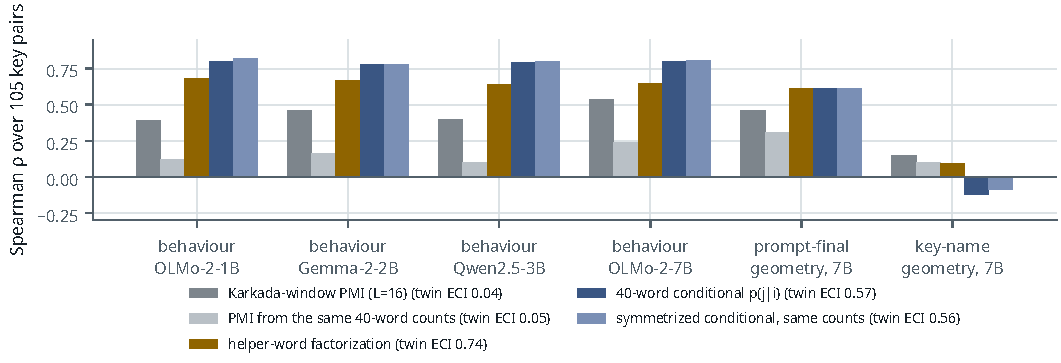
\includegraphics[width=.96\linewidth,keepaspectratio]{figures/fig_operators.pdf}
\kirinfigcaption{Figure 4.}{Which operator predicts which observable. Spearman correlation between each operator's pairwise distances and those of the observable (restricted next-key behaviour in the modulation family, four models; 7B prompt-final and key-name geometry). Association operators (greys/gold): Karkada-window PMI, a PMI built from the same 40-word counts as the conditionals, and the helper-word factorization. Conditional-row operators (blues): the directional 40-word conditional and a symmetrized conditional from the same counts. Twin ECI in the legend: mean percentile rank of the three enharmonic pairs (0 = closest, 0.5 = null).}
\end{minipage}

\begin{resultbox}[{Result 4 --- the contrast is conditional-row vs association, not directional vs symmetric}]
Geometry over the 15 spellings: Karkada-window PMI puts twins closest (ECI $0.04$; controlled \cl{} $+0.42$, \lc{} $+0.39$) and so does the PMI built from the 40-word counts (ECI $0.05$; \cl{} $+0.62$, \lc{} $+0.14$); every conditional-row operator keeps them apart --- directional ECI $0.57$, symmetrized $0.56$, reverse $0.60$ (controlled \cl{} $+0.55$/$+0.55$/$+0.56$, \lc{} $+0.12$/$+0.18$/$+0.18$) --- while remaining fifths-periodic under control; the helper factorization keeps them farthest (ECI $0.74$; \cl{} $+0.21$, \lc{} $-0.07$). Predicting next-key behaviour in the modulation family (Spearman over 105 pairs; OLMo-1B/Gemma/Qwen/OLMo-7B): directional conditional $+0.80/{+}0.78/{+}0.79/{+}0.80$; symmetrized conditional from the same counts $+0.82/{+}0.78/{+}0.80/{+}0.81$; reverse conditional $+0.83/{+}0.78/{+}0.80/{+}0.81$; helper factorization $+0.68/{+}0.67/{+}0.64/{+}0.65$; Karkada-window PMI $+0.39/{+}0.46/{+}0.40/{+}0.54$; PMI from the same 40-word counts $+0.12/{+}0.16/{+}0.10/{+}0.24$. Predicting the 7B prompt-final geometry: conditionals $+0.60$--$0.61$, helper $+0.61$, Karkada PMI $+0.46$, 40-word PMI $+0.31$. Predicting key-name span-mean geometry: nothing above $+0.15$ (helper $+0.37$ for Qwen). The document-conditional rows, though conditional and directional, predict none of the three observables as a \emph{similarity} (nothing above $+0.14$; $-0.07$ to $+0.03$ for behaviour); their residuals nevertheless carry the largest held-out gain (\S\ref{sec:heldout}). As \emph{held-out regressors} (\S\ref{sec:heldout}, target-aggregated modulation family) the matched operators rank the same way but less sharply: symmetrized conditional $\Delta\KL=+0.039/{+}0.030/{+}0.016/{+}0.040$, directional $+0.037/{+}0.029/{+}0.016/{+}0.036$, reverse $+0.029/{+}0.027/{+}0.013/{+}0.030$, PMI from the same counts $+0.021/{+}0.014/{+}0.012/{+}0.029$ (all $p\le.001$) --- the association construction retains half to three quarters of the conditional's gain as a regressor, because as a single column it differs from the symmetrized conditional only by a target-marginal term that the theory features partly absorb.
\end{resultbox}

This is the descriptive statement of operator-dependent geometry, and the matched control sharpens it: what separates the operators that align with behaviour from those that do not is the construction --- a row-conditional of local co-mentions with row-divergence geometry, versus an association statistic normalized by marginals --- not directionality (the symmetrized and reversed conditionals do as well as the directional one) and not the window (the 40-word PMI does worse than the $L=16$ PMI). The local conditional is the operator most closely aligned with the next-key behavioural task among those tested; it is not literally the next-token objective. This is a comparison of operators computed from one corpus against models trained on others; it does not test either theory's factorization claim, and we do not read it as ``Karkada predicts circle, Zhao proves line''. We have no tested explanation for the document conditional's paradox (poor similarity, strong residual regressor); the natural conjecture --- offered as such, untested here --- is that document co-occurrence is dominated by topical and genre structure nearly orthogonal to the theory features, which makes it a poor \emph{similarity} and a good \emph{regressor}. The Gemma column was added at the hardening stage; no new forward passes were needed.

\section{Held-out prediction beyond theory geometry}\label{sec:heldout}

Result 4 could still be ``both matrices look like the line''. The central test asks whether the corpus conditionals predict model behaviour \emph{after} the explicit geometric and orthographic explanations are removed, on held-out rows. It was pre-registered before any Phase-V comparison was run.

\paragraph{Objects} $Q^{(m,f)}$: model $m$'s $15\times15$ behavioural matrix in family $f$. $C^{(c,F)}$: corpus $c$'s conditional under extraction family $F$ --- A: directional 40-word window; B: window with an intervening cue (modulation, chord, key signature, enharmonic, relation); C: high-precision regexes (``from X major to Y major'', 317 pairs, too sparse to use); D: document-conditioned, $j$ anywhere later in the document than $i$. Add-0.5 smoothing, row-normalized; Wikipedia yields 47,247 (A), 10,775 (B), 19,162 (D) ordered pairs from 9,168 key-mentioning documents (the Phase-I helper-word factorization of Result~1 used a wider pass over 14,235 documents containing any of the 42 major- and minor-key spellings; the conditional scan is restricted to the 15 major-key spellings).

\paragraph{Theory features} Per ordered pair $(i,j)$: circle distance, line distance, signed difference $s_j-s_i$, glyph-class equality, has-accidental of source and target, root-letter identity, edit distance, log source and target frequency, token counts. The \emph{rich} variant adds quadratics, the product circle$\times$line and cosine harmonics $\cos(2\pi k\,d_c/12)$, $k=1,\dots,3$.

\paragraph{Tests} (1) Residual correspondence: ridge-regress $\log Q$ and $\log C$ on the features, Spearman of the residuals, joint key-relabeling null (2000). (2) Leave-one-source-row-out prediction of $Q$ with theory-only, corpus-only and theory+corpus predictors, scored by within-row Spearman (the pre-registered rank scorer $\Delta$CV), by softmax-KL of the predicted row against the actual row (pre-registered in the design but --- see Appendix~A --- implemented only after the rank scorer had been seen to be null), and by the within-row $R^2$ gain; relabeling null ($B=5{,}000$, $p=(b+1)/(B+1)$) and a document-cluster bootstrap (300 resamples; Appendix~D.6). The hold-out is over \emph{source rows}, not over prompt templates: the four templates of a family are averaged in log-probability before the analysis. Template robustness (Appendix~C.7): the flagship gain is significant in every leave-one-template-out aggregate for all four models ($\Delta\KL$ $+0.026$…$+0.051$ window, $+0.030$…$+0.052$ document, $p\le.0005$) and in three of the four single templates; the fourth (``originally in \{x\} major, was later transposed to'') gives smaller gains that are n.s.\ for Qwen and OLMo-7B. (3) Enharmonic-twin difference vectors, raw and line-controlled. Two views throughout: the spelled view (15 targets) and the 12-class target-aggregated view, in which the target columns of the already-scored candidate distribution are merged into pitch classes by log-sum-exp and class-level features are used. This is a diagnostic projection of the prediction space, not a scoring rule for the modulation task: it removes target-spelling and seam structure so that the question ``does corpus-specific structure still predict behaviour?'' is asked under a stringent deconfounding; it should not be confused with the enharmonic-merged behavioural scorer of \S\ref{sec:setup}, which applies to families B--D only.

\par\vspace{4pt}
\noindent\begin{minipage}{\linewidth}
\centering
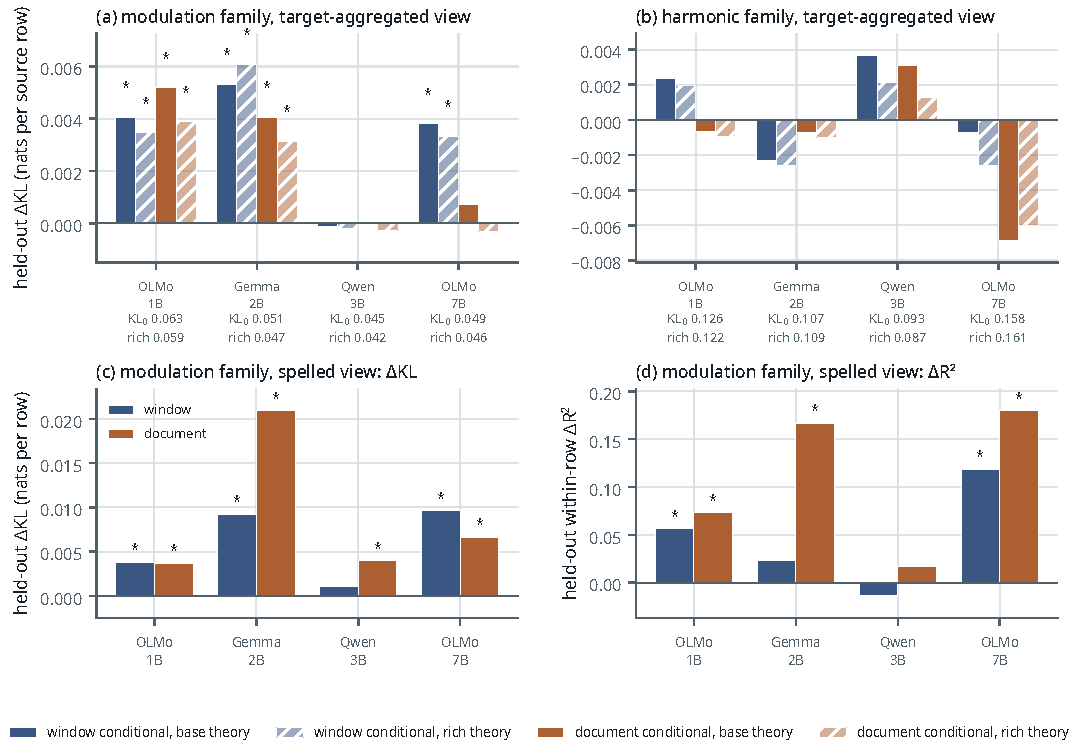
\includegraphics[width=.96\linewidth,keepaspectratio]{figures/fig_heldout.pdf}
\kirinfigcaption{Figure 5.}{Held-out gain from the corpus conditionals beyond the theory model, Wikipedia. (a, b) Target-aggregated view: reduction in held-out KL per source row when the corpus row is added to the theory features, for the window (blue) and document (orange) conditionals, with the base (solid) and rich (hatched) theory model; each tick label gives the base and rich theory-only held-out KL, and hatched bars should be read against the rich value; $*$: relabeling $p<.05$; (a) modulation family, (b) harmonic-relation family. (c) Spelled view, modulation family, held-out $\Delta\KL$; (d) the same cells scored by within-row $\Delta R^2$ --- the two scorers agree throughout the target-aggregated view and only partly in the spelled view. Numbers in Appendix~C.}
\end{minipage}

\begin{resultbox}[{Result 5 --- the central number}]
\textbf{Target-aggregated view, modulation family} (OLMo-1B/Gemma/Qwen/OLMo-7B). Adding the corpus row to the theory model reduces held-out KL by $+0.037/{+}0.029/{+}0.016/{+}0.036$ nats per row (window conditional) and $+0.045/{+}0.036/{+}0.023/{+}0.039$ (document conditional) against a theory-only KL of $0.117$--$0.134$ --- a 14--34\% reduction; relabeling $p\le8\times10^{-4}$ in every cell and $b=0$ of $5{,}000$ ($p\le2\times10^{-4}$) in six of eight; within-row $\Delta R^2=+0.29/{+}0.30/{+}0.19/{+}0.33$ (window) and $+0.36/{+}0.38/{+}0.24/{+}0.38$ (document). Document-cluster bootstrap 95\% intervals (9,168 documents resampled, 300 draws) exclude zero in every cell: window $[+0.020,+0.040]$, $[+0.017,+0.032]$, $[+0.007,+0.020]$, $[+0.018,+0.038]$; document $[+0.009,+0.049]$, $[+0.010,+0.037]$, $[+0.0003,+0.024]$, $[+0.008,+0.040]$. \textbf{Rich theory model:} $\Delta\KL=+0.023/{+}0.019/{+}0.007/{+}0.018$ (window; $p=.0006/.0004/.013/.0002$) and $+0.034/{+}0.026/{+}0.013/{+}0.022$ (document; $p=.0004/.0002/.003/.0008$), a 6--28\% reduction of the rich model's own $\KL_0$ ($0.105$--$0.123$); $\Delta R^2$ $+0.17/{+}0.18/{+}0.06/{+}0.18$ and $+0.26/{+}0.29/{+}0.11/{+}0.24$. \textbf{Training-row target prior:} with each target's mean log-probability over the 14 training rows added to the theory model (recomputed inside every fold), the gain is \emph{larger}, not smaller: $+0.041/{+}0.035/{+}0.025/{+}0.047$ (window) and $+0.047/{+}0.042/{+}0.031/{+}0.049$ (document), all $p\le2\times10^{-4}$; with the rich model as well, $+0.027/{+}0.022/{+}0.011/{+}0.025$ and $+0.035/{+}0.029/{+}0.018/{+}0.029$, all $p\le8\times10^{-4}$. The corpus therefore predicts source-specific conditional structure, not the models' generic preference for popular target keys. \textbf{Residual correspondence} (not held-out): $+0.60/{+}0.59/{+}0.50/{+}0.60$ for the document conditional ($p\le8\times10^{-4}$), $+0.53/{+}0.52/{+}0.39/{+}0.51$ under the rich model. \textbf{Harmonic-relation family:} base-model gains ($\Delta\KL$ $+0.024/{+}0.000/{+}0.024/{+}0.039$, $p=.026/.55/.056/.004$) vanish under the rich model ($p\ge.21$) but reappear once the target prior is included ($+0.032/{+}0.007/{+}0.042/{+}0.058$, $p\le.005$; rich $+0.013/{-}0.000/{+}0.019/{+}0.018$, three of four $p\le.001$). \textbf{Chord family:} OLMo-7B ($\Delta\KL$ $+0.064/{+}0.071$ of $0.357$, $p\le.002$) and marginally Qwen ($+0.016/{+}0.017$, $p=.036/.050$); Gemma and OLMo-1B null. \textbf{Spelled view:} theory-only leave-one-out Spearman is already $0.78$--$0.95$ because the rows are line-dominated. The $R^2$ scorer shows a gain (modulation$\times$window $+0.10$, 1B, $p=.015$; $+0.22$, 7B, $p\le2\times10^{-4}$; $\approx+0.02$ for Gemma and Qwen, n.s.; modulation$\times$document $+0.14/{+}0.12/{+}0.05/{+}0.30$, Qwen n.s.), \emph{but the KL scorer confirms it in only three of eight cells}: $\Delta\KL$ is $+0.012$ nats at most, significantly positive for 1B$\times$window ($+0.006$, $p=.009$), Gemma$\times$document ($+0.012$, $p=.009$) and 7B$\times$window ($+0.007$, $p=.001$) against a spelled theory KL of $0.05$--$0.07$, and null or slightly negative in the other five, including OLMo-7B$\times$document ($-0.002$) where $\Delta R^2$ is largest. The two scorers agree throughout the target-aggregated view and only partly in the spelled view.
\end{resultbox}

\begin{auditbox}[{Audit note --- pre-specification, multiplicity and the two scorers}]
No single cell of the model $\times$ family $\times$ extraction grid was pre-specified as primary; the design listed all three context families and four extraction families as competing hypotheses and the ``central number'' as the held-out gain across them. All 36 cells of each view are reported (Appendix~C.2, Figure~5), and the modulation family is emphasized \emph{post hoc} because it is the only family whose gain survives the rich theory model in all four models. Cell-level $p$-values are unadjusted structured-null values; the flagship cells have $b=0$ of $B=5{,}000$ relabelings ($p\le2\times10^{-4}$), which survives a Bonferroni factor of 36, whereas the rich-model $p$-values of $.003$--$.017$ do not, and we lean on replicated effect direction and size across the four models rather than on any adjusted threshold.\par\smallskip

The pre-registered rank scorer $\Delta$CV (within-row Spearman over the 11--14 targets of a held-out row) was $\approx0$ in the same cells (between $-0.026$ and $+0.011$; significant in the target-aggregated view only for OLMo-7B, five cells at $+0.028$…$+0.087$, and Gemma, two modulation cells at $+0.020/{+}0.022$, all $p\le.008$ at $B=5{,}000$). The design document had also named a softmax-KL scorer, but only the rank scorer was implemented in the first run. The KL scorer, and a within-row $R^2$ gain that the design had not named, were implemented \emph{after} the gap between residual $r\approx0.5$--$0.6$ and $\Delta\mathrm{CV}\approx0$ had been seen. A further correction was made at the hardening stage: the first implementation used 300 relabelings and the estimator $b/B$, which cannot resolve below $0.0033$, yet the draft reported ``$p<.001$''; every Phase-V $p$-value was recomputed with $B=5{,}000$ (Wikipedia) or $2{,}000$ (other corpora, checkpoints) and the finite-sample estimator $(b+1)/(B+1)$. The flagship cells have $b=0$ of $5{,}000$. The reason is distributional --- a rank metric over eleven targets discards most of the probability mass that the corpus re-weights --- and the result was then subjected to the same permutation nulls and to the rich-theory model. Both scorers are reported; the KL result should be read as pre-registered in content and post-hoc in timing.
\end{auditbox}

Twin difference vectors ($\log q(\cdot\mid$C\fl$)-\log q(\cdot\mid$B$)$ etc.) correlate strongly with their corpus counterparts for the rarest twin (C\fl$|$B cosine $+0.65$…$+0.92$; G\fl$|$F\sh{} $+0.41$…$+0.86$; D\fl$|$C\sh{} only $+0.02$…$+0.54$), but that is the line; after residualizing both on the target's line position and glyph class, significant alignment survives in seventeen of the 108 cells --- more than the five expected by chance, but scattered (e.g.\ OLMo-1B C\fl$|$B $+0.74$, $p=.01$; Gemma D\fl$|$C\sh{} $+0.79$, $p<.005$; Qwen G\fl$|$F\sh{} $+0.89$, $p<.001$; 7B $+0.71$, $p=.02$) with no consistent pattern across extraction or context families. We do not build on it.

\section{The gain is generic across corpora; corpus specificity is inconclusive}\label{sec:cross}

The residual correspondence of Result 5 is present in four models trained on four different corpora, so on Wikipedia alone it is a property of how English text about keys is written, not evidence about any model's data. We tested the stronger reading directly on the data OLMo-2 actually consumed \citep{olmo2,dclm2024}: the OLMo-Mix-1124 wiki (both shards; the Dolma wiki, whose documents are three times shorter than the 2023 dump --- 6,857 key documents, 8,540 window pairs), a 9-shard OLMo-Mix DCLM sample ($\approx0.02\%$ of DCLM; 386 key documents, 633 window pairs), a 54-shard OLMo-Mix DCLM sample scanned after the first analyses (2,884 documents, 3,843 pairs), a 2-shard Dolmino DCLM sample (611 documents, 1,320 pairs) and Dolmino FLAN (49 documents, 6 pairs, unusable). Each corpus is compared with Wikipedia binomially thinned to the same pair mass per extraction family, and specificity is the difference-in-differences (DiD) of per-row held-out $\Delta\KL$: (OLMo models $-$ Gemma/Qwen) $\times$ (corpus $-$ size-matched Wikipedia), Wilcoxon over the 15 source rows, for all nine pre-registered cells per corpus (three context families $\times$ the window, cue and document extractions) and both views. An earlier draft of this section, and the repository's Phase-V results file before correction, reported only the four harmonic/modulation $\times$ window/document cells; that restriction was post-hoc and is withdrawn (Appendix~A).

(Per-cell values are plotted in Figure~C.1 and tabulated in Appendix~C.3.)

\begin{resultbox}[{Result 6 --- generic gain; specificity inconclusive}]
Every corpus adds held-out value for every model in the modulation family: even the 633-pair DCLM sample gives $\Delta\KL=+0.037/{+}0.029/{+}0.030/{+}0.047$ ($p\le.019$, $B=2{,}000$), and at 3,843 pairs the within-row $\Delta R^2$ is $+0.18/{+}0.13/{+}0.15/{+}0.19$ for the window conditional ($p\le.0015$), though its $\Delta\KL$ ($+0.021/{+}0.010/{+}0.017/{+}0.024$) reaches significance only in the 7B ($p=.005$) --- the theory KL is inflated to $0.17$--$0.21$ there because DCLM frequency features are poor. In the smallest samples the real web corpora beat size-matched Wikipedia for all four models (633-pair OLMo-Mix DCLM, document conditional: $+0.024/{+}0.025/{+}0.025/{+}0.030$ nats above thinned Wikipedia), a genre effect shared by OLMo and non-OLMo models; at 3,843 pairs the comparison is mixed (document conditional above thinned Wikipedia by $+0.008$…$+0.011$; window conditional below it for three of four models, by $0.007$--$0.016$, and marginally above for Qwen, $+0.002$), so we do not build on it. \textbf{Specificity.} Over all 36 target-aggregated and 36 spelled DiD cells (Appendix~C.3), 10 reach $p<.05$ and all 10 are positive, i.e.\ OLMo-favouring: on OLMo-Mix wiki, harmonic$\times$window ($+0.007$, $p=.01$), harmonic$\times$cue ($+0.015$, $p<.005$) and modulation$\times$document ($+0.008$, $p=.04$) in the target-aggregated view and the same three cells in the spelled view; on the 9-shard DCLM sample, spelled modulation$\times$window ($+0.005$, $p=.01$); and chord$\times$document on both DCLM corpora OLMo consumed (Dolmino $+0.049$, $p<.005$; 54-shard OLMo-Mix $+0.023$, $p=.01$), plus Dolmino chord$\times$window in the spelled view ($+0.017$, $p=.02$). Against this: the effects are small relative to the gains ($0.004$--$0.05$ vs $0.03$--$0.07$ nats); six of the ten separate both OLMo models from both others, but four are carried by OLMo-2-7B alone and Gemma outgains an OLMo model in two; the modulation family that carries this paper's main result shows DiD $\approx0$ on every DCLM sample in the target-aggregated view ($-0.014$…$+0.010$, $p\ge.09$); 34 of the 72 cells are negative (36 positive, 2 zero); the 72 tests are not multiplicity-corrected; and the cells are far from independent --- the spelled and target-aggregated views are two readings of the same fifteen rows, and three of the ten significant cells are one such pair each, so the ten reduce to seven distinct corpus $\times$ family $\times$ extraction combinations. We therefore report the specificity test as \emph{inconclusive}: seven distinct significant combinations all pointing the same way is more than a pure null comfortably produces, but no cell replicates across corpora within the family where the gain is robust, and the corpus that is 95\% of OLMo's stage-1 tokens shows nothing there in the target-aggregated view at either sample size, its single significant spelled modulation cell at 633 pairs ($+0.005$, $p=.01$) failing to replicate at 3,843 pairs ($p=.76$).
\end{resultbox}

We therefore state the claim as ``conditional natural-language statistics predict behaviour across models''; we neither claim that behaviour recovers the training set nor that it does not. Caveats: even the larger DCLM sample is $\approx0.1\%$ of DCLM, the paired test has fifteen rows of power, and frequency features are recomputed per corpus so theory KLs differ across corpora (the size-matched baseline shares that handicap).

\section{Two artifact explanations, tested causally}\label{sec:synthetic}

Two cheap explanations of the natural line remained after \S\ref{sec:behaviour}: that spelled output tokens alone deform prediction over a periodic statistic, and that models are frozen mid-way through learning rare enharmonic equivalences. Both were tested with from-scratch transformers (4 layers, $d=128$) on synthetic data with no music vocabulary: 15 source states $n=-7..+7$, latent classes $z=n \bmod 12$ (three duplicated labels), a shared query token whose residual is the predictive-state probe, and eight-symbol output codewords.

\par\vspace{4pt}
\noindent\begin{minipage}{\linewidth}
\centering
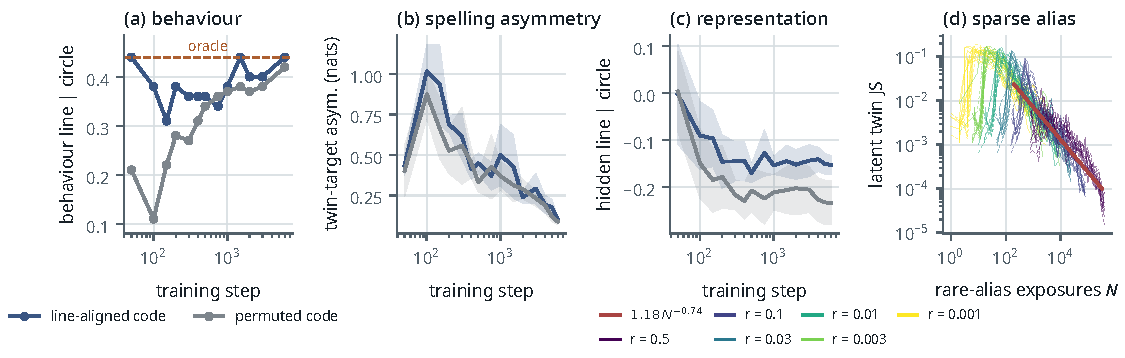
\includegraphics[width=.96\linewidth,keepaspectratio]{figures/fig_synthetic.pdf}
\kirinfigcaption{Figure 6.}{Synthetic controls. (a--c) Periodic (CIRCLE) law, line-aligned vs permuted output code, five paired seeds: behaviour (\lc{} without code control, seed means) reaches the oracle's own value faster under the aligned code and ends at the same value (a); the spelling asymmetry between twin targets is transiently larger and vanishes (b, mean $\pm$ sd); the predictive-state representation keeps a small persistent \emph{relative} shift toward the line under the aligned code, both partials remaining negative and below their relabeling nulls (c, last layer, mean $\pm$ sd; the headline $+0.097$ contrast is at the mid layer). (d) Sparse source aliases: latent twin divergence collapses onto one power law in cumulative rare-alias exposures across rarity levels $r$ (solid: aligned code; dashed: permuted).}
\end{minipage}

\begin{resultbox}[{Result 7 --- output-code geometry: transient in behaviour, small and persistent in representation}]
$2\times2$ factorial, \{CIRCLE, LINE\} law $\times$ \{line-aligned, permuted\} code, five paired seeds, entropy-matched oracles (2.137 nats). All 20 runs reach KL $\le0.001$ to their oracle. Under the periodic law, converged behaviour is periodic in both code conditions (\cl{} $0.98$; \lc{} $0.436$ vs $0.422$ against the oracle's own $0.439$; twin-target asymmetry $+0.013$, i.e.\ $\approx1\%$, 5/5 seeds, $p=.044$). Early in training the aligned code is closer to the oracle (KL $0.078$ vs $0.276$ at step 100) and twin asymmetry is larger through step $\approx1500$; all behavioural differences vanish by step 500--2000, and dose-response over five alignment levels gives Spearman $+0.85$ for the early behavioural line and $-0.68$ for early KL. The predictive-state representation keeps a $+0.08$…$+0.10$ shift toward the line (5/5 seeds, $p=.001$ mid-layer) --- a paired \emph{difference}: the absolute partial stays negative in both conditions ($-0.15$ vs $-0.23$ at the last layer) and below each run's relabeling-null 95th percentile ($+0.17$…$+0.21$), so neither condition has a significant line --- and a code-imprinted quadratic bow ($|\rho(\mathrm{PC}_2,(n-\bar n)^2)|=0.85$ vs $0.39$). Positive control: an arbitrary code does not hide a true line ($0.995$ recovered), though its bent open embedding registers as a spurious \cl{} partial ($+0.32$) --- another instrument caution.
\end{resultbox}

\begin{resultbox}[{Result 8 --- sparse aliases: rarity, not symmetry}]
Source-alias rarity $r\in\{0.5,\ldots,0.001\}$ with latent-class mass and target law fixed (natural Wikipedia ratios: C\fl:B $=0.024$, C\sh:D\fl $=0.22$, G\fl:F\sh $=0.41$), 91 runs. Global KL stays at the floor ($0.001$--$0.007$) while rare rows carry 3--24$\times$ the error, so aggregate metrics do hide an unresolved alias --- but the residual shrinks monotonically. Pooling 1,254 checkpoints, latent twin JS $\approx1.18\,N^{-0.74}$ in cumulative rare exposures $N$ (partial Spearman with exposure given step $-0.84$; with step given exposure $-0.19$), and exposure-matched medians coincide across $r$. The aligned code \emph{lowers} the error at every sparse $r$ (significantly at $r=.01$, $p=.02$, and $r=.001$, $p=.035$; same sign but n.s.\ at $r=.003$, $p=.16$; power-law prefactor $0.94$ vs $1.5$ at a common exponent). An equally rare unique state is learned about as well as the rare alias at matched exposure ($r=.01$: row KL $0.0064$ at 2.6k exposures vs $0.0105$ at 2.3k), so nothing transfers the twin's row to the rare alias; and the representational twin distance collapses after $\approx250$--$2{,}400$ rare exposures whereas behavioural equalization needs $\approx0.8$k--$7.7$k, the representational threshold coming first in every run where both are crossed except one. This is the ordinary long-tail regime \citep{kandpal2023longtail}, not a symmetry-specific bottleneck. Separately, the natural premise fails: Wikipedia's next-key rows for C\fl{} and B are not the same predictive state (latent JS $0.228$, 81st percentile of all pairs).
\end{resultbox}

Together: spelled outputs are sufficient for a weak representational tilt, faster acquisition and transient behavioural bias, and insufficient for the converged natural line; rare-alias learning is ordinary sample complexity with no symmetry-specific bottleneck. These two mechanisms --- output-code geometry alone, and sparse-alias learning --- are insufficient for the natural line; other lexical or learning explanations are not thereby excluded, but the two most economical ones are, which is why \S\ref{sec:heldout} could treat the line as data structure.

\section{Acquisition along one pretraining run}\label{sec:trajectory}

OLMo-2-0425-1B publishes intermediate checkpoints. We scored eight stage-1 revisions (1B, 21B, 49B, 105B, 294B, 1007B, 1993B, 4001B tokens) and all three stage-2 ingredient endpoints (51B tokens each, same stage-1 start, different seeds) with the behavioural battery, and computed for each the line/circle partials and the target-aggregated residual correspondence with Wikipedia conditionals under the rich theory model (2,000 relabelings, $(b+1)/(B+1)$); \S\ref{sec:cross} showed that this residual is not specific to any one corpus, so ``residual correspondence'' below means correspondence with conditional statistics beyond the theory features.

\par\vspace{4pt}
\noindent\begin{minipage}{\linewidth}
\centering
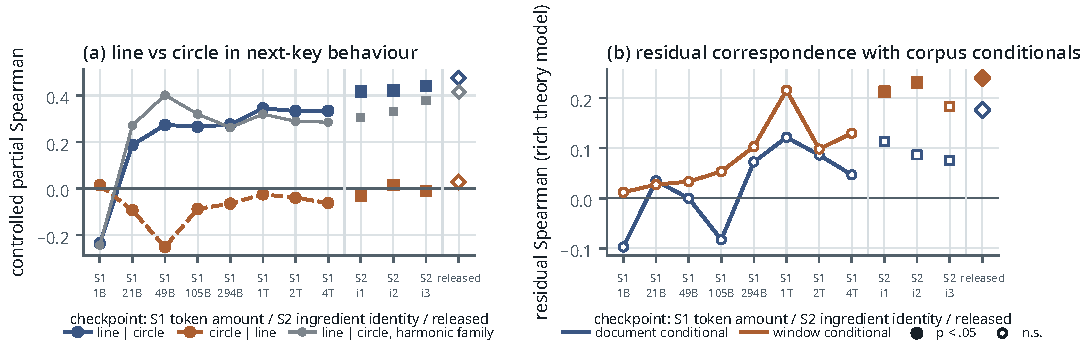
\includegraphics[width=.96\linewidth,keepaspectratio]{figures/fig_trajectory.pdf}
\kirinfigcaption{Figure 7.}{OLMo-2-1B checkpoints, modulation family. (a) The open-line coordinate appears by 21B tokens and rises in two steps (blue; grey: the same partial in the harmonic-relation family); the circle partial (orange) stays near zero apart from a single excursion to $-0.25$ at 49B tokens. (b) The residual correspondence with Wikipedia conditionals emerges later and noisily: first $p<.05$ at 294B tokens, a dip at 1T, stable from 4T; filled markers $p<.05$ ($B=2{,}000$ relabelings). Squares: the three stage-2 seeds; diamond: the released model, which is a different training run (text).}
\end{minipage}

\begin{resultbox}[{Result 9 --- coarse structure early, residual correspondence later}]
\lc: $-0.24$ (1B tokens) $\to$ $+0.19$ (21B) $\to$ $+0.27$ (49--294B) $\to$ $+0.34$ (1T) $\to$ $+0.33$ (2T, 4T) $\to$ $+0.42/{+}0.42/{+}0.44$ (stage-2 seeds); \cl{} $\approx0$ throughout. Residual correspondence, document conditional ($B=2{,}000$ relabelings): $+0.15$ (n.s.) $\to$ $+0.27$ (105B, $p=.10$) $\to$ $+0.40$ (294B, $p=.037$) $\to$ $+0.26$ (1T, $p=.23$) $\to$ $+0.34$ (2T, $p=.050$) $\to$ $+0.44$ (4T, $p=.005$) $\to$ $+0.48/{+}0.45/{+}0.46$ (stage 2, $p\le.017$). Twin asymmetry falls from $4.3$ nats (rare spellings nearly unlearned) to $2.6$; twin-difference directions stabilize by 49B tokens. Stage 2 --- the Dolmino mix, which multiplies the Wikipedia share by $\approx75$ --- raises the line by $+0.09$…$+0.11$ in 3/3 seeds and changes the residual correspondence by $+0.01$…$+0.04$, within replicate spread.
\end{resultbox}

This is one run, one family with a clean signal, an unexplained dip at 1T, and no reconstructible data order (none is published for the 1B; only the 32B has official OLMo-core scripts), so it is suggestive, not a law.

\paragraph{Provenance of the released 1B model} One finding matters for anyone using these checkpoints: the released \texttt{OLMo-2-0425-1B} weights are orthogonal to every branch checkpoint (cosine $\approx0.00$ for attention, MLP and unembedding matrices, singular values $\approx2.2\times$ larger, identical configuration) while the three ingredient endpoints are cosine $0.96$--$1.0$ to the stage-1 endpoint. The released model is a different training run, not the trajectory's endpoint and not a soup of the ingredients; it is plotted as a separate point (\lc{} $+0.47$, residual $+0.53$), which mildly strengthens replication and complicates provenance.

\section{Discussion}\label{sec:discussion}

\paragraph{One concept, several geometries} There is no context-free geometry of musical keys waiting to be read from either language statistics or activations. PMI-type association strongly identifies enharmonic twins and carries robust periodic fifths structure, which Wikipedia exhibits and which a Karkada-style helper-vocabulary factorization reproduces. Conditional-row operators preserve distinctions between spelled tonal states, because C\fl{} major and B major occur in different linguistic contexts and are followed by different keys --- and it is these operators, symmetrized or directional, that align with the models' restricted next-key behaviour, ordering \emph{local conditionals $>$ helper factorization $>$ Karkada-window PMI $>$ 40-word PMI $\approx$ document conditional}. The matched control shows the ordering is a property of the construction, not of directionality or window width. Hidden-state geometry, meanwhile, is dominated by lexical structure that projects onto the very harmonics used to diagnose semantic symmetry. In this domain a geometric interpretation is meaningful only relative to the operator, the equivalence relation, the measurement location and the task that define it; one domain does not establish a law, but the paper identifies quantitatively which operator predicts which observable.

\paragraph{Why orthography is not simply nuisance} Under \citet{temperley2000line} and \citet{moss2023line} spelling is part of tonal semantics; treating it as a covariate reveals a periodic corpus, treating it as the coordinate reveals an open one. We report both throughout (spelled and target-aggregated views) and privilege neither. What we do claim is that removing spelling, circle, line and frequency \emph{jointly} still leaves structure in the corpus conditionals that predicts held-out behaviour.

\paragraph{Methodological implications} Three instrument lessons generalize beyond music. A categorical feature contiguous on the chosen cyclic ordering fakes the fundamental of the competing ordering, and the standard months/weekdays Fourier pipeline reported the key-name geometry as a circle; the cure is to project out (or respell away) candidate categorical features and to report mode isotropy --- with the caveat that our two anisotropy diagnostics are not fully concordant here (isotropy $0.4$--$0.65$ reads as a $15$--$30\%$ circle admixture where the projection-matched $P_5$ diagnostic reads $0$--$15\%$, and isotropy is uncalibrated for anisotropic residual noise) and that spectral sparsity does not guarantee separability \citep{fu2026convergent}. The last token of a multi-token concept name is not a neutral probe when token types differ across concepts, and neither is the span mean; the shared prompt-final position is. And a rank-based held-out scorer over a dozen targets can miss a distributional gain of a third of the residual KL. The recipe generalizes: any concept family whose surface form is contiguous on the ordering one Fourier-analyses will produce this false positive, and the test is a respelling or projection intervention, not a larger model.

\paragraph{Relation to the two theories} Karkada's construction is theory for embedding models and their LLM evidence is qualitative; Zhao et al.'s geometry is a statement about support patterns that are degenerate at this vocabulary size. Our results are empirical alignments between operators and observables, consistent with the qualitative idea that recovered geometry depends on which statistical object the computation is aligned with. We have not tested either factorization claim and do not manufacture a unification.

\paragraph{Limitations} One semantic domain, chosen because it is unusually structured; generalization to other families with competing quotient geometries is untested. The behavioural task is constructed (next-key prompts, four templates per family), not unrestricted language use. The corpora are proxies even for OLMo (samples of DCLM; Gemma and Qwen data are unavailable), and the cross-corpus test has fifteen paired rows of power. The target-aggregated view merges targets and thereby changes the task; in the spelled view the $R^2$ and KL scorers disagree and only the former shows a gain. The KL scorer's timing is post-hoc (Audit note). Correspondence between corpus conditionals and behaviour is not causation: the synthetic studies show sufficiency and insufficiency of two alternatives, not that these statistics built the behaviour. The checkpoint evidence is one run whose released endpoint is a different run. Hidden-state claims are weak by design; the cleanest result is behavioural and statistical.

\paragraph{Why the failed hypotheses are in the paper} The initial analysis was wrong in the obvious way; the ``circle-to-line transition'', ``predicting-position locus'', ``scaling trend'' and ``black/white-key feature'' readings were killed by matched contexts, layer-selection nulls, a respelling intervention and two model-assisted audit passes; the lexical-code and frozen-transient explanations were killed by experiment; the training-data fingerprint could not be established (and, after the full cell set was examined, could not be excluded either). The final claim is the one that survived all of that; the controls and falsification experiments are the evidence, and the audit trail (Appendix~A) records what was tried.

\section*{Reproducibility}
All code, results files, figures and logs are in the public repository \href{https://github.com/VykosMolt/One-Concept-Multiple-Geometries}{\mbox{\texttt{github.com/VykosMolt/}}\allowbreak\mbox{\texttt{One-Concept-Multiple-Geometries}}} (tag \texttt{paper-v1}); model weights, corpora and the extracted hidden-state tensors are excluded from the mirror and listed with sizes and SHA-256 digests in its \texttt{MIRROR\_MANIFEST.md}. The chronological logs (\mbox{\texttt{RESEARCH\_LOG.md}}, \mbox{\texttt{PHASE2\_LOG.md}}--\mbox{\texttt{PHASE5\_LOG.md}}) state, for each analysis, whether it was fixed before or after the relevant data were seen; the design documents (\mbox{\texttt{PHASE3\_DESIGN.md}}--\mbox{\texttt{PHASE5\_DESIGN.md}}) were written before any run of their phase. Figures in this paper are regenerated from the results files by \texttt{paper/make\_figs.py}. Compute: one RTX~5070~Ti laptop GPU; forward passes only for the natural models; the synthetic runs take $\approx40$~s each.

\bibliography{refs}

\clearpage
\kirinappendixstyle
\kirinpart{Appendix A}{Audit trail: retracted claims and post-hoc decisions}

Two independent model-assisted adversarial audit passes (a code and instrument verification; a scientific review), and three further model-assisted audits of the manuscript, were run; these are not human peer review and are not offered as a credential --- their verbatim summaries are in the repository (\texttt{notes/review\_code.md}, \texttt{notes/review\_science.md}, \texttt{MANUSCRIPT\_AUDIT.md}). The table lists every claim that was made during the project and later withdrawn, with what killed it, and every analysis decision that was taken after seeing data.

\begin{longtable}{@{}p{0.30\linewidth}p{0.14\linewidth}p{0.50\linewidth}@{}}
\toprule
\kirintablehead{Claim or decision} & \hd{Status} & \hd{What happened} \\
\midrule
\endhead
Key-name activations contain a circle of fifths ($P_5$ share $0.33$, $z\approx3.7$) & \statusRetracted & Accidental-indicator projection: $P_5$ falls to the matched null; respelling shows the block is orthographic (\S\ref{sec:alias}). \\
``Projected $P_5$ is below the null'' & \statusCorrected & The projection-matched null is $0.120$, not $2/11$; observed $0.11$--$0.14$ is \emph{at} the null ($z=+0.4$). \\
``Projection removes 13.5\% of a circle's energy'' & \statusCorrected & It removes 47.9\% of the \emph{energy} (13.5\% of the share); the projection is not mild, the share-based conclusion stands. \\
Black/white-key semantic block & \statusRetracted & Respelling C, E, F, B as B\sh, F\fl, E\sh, C\fl{} moves the block with the glyph in all four models. \\
Fifths geometry scales with model size & \statusRetracted & With max-over-layers nulls three of four points are at $p=0.09$--$0.25$; only the 7B is significant. \\
The circle lives at the predicting position & \statusRetracted & Matched contexts: concept token $+0.33$…$+0.52$ vs predicting token $+0.38$…$+0.53$; the difference was context, not position. \\
Circle mid-network, line at the output & \statusRetracted & Significant in 1 of 12 model$\times$context cells after correction. \\
Line in key-name geometry of Qwen/7B (six families) & \statusRetracted & Carried by the accidental token being the last token of two-token keys; $\approx0$ under a span-mean probe. \\
Modulation context strengthens the line at the key token & \statusRetracted & Same last-token artifact ($+0.21\to-0.10$ at span mean); prompt-final effects retained (small). \\
Separable circle/line/spelling subspaces (H5) & \statusUnresolved & Cross-fitted subspaces overlap; variance shares sum above one. \\
Arbitrary output codes carry the line (Phase II) & \statusRetracted & First pass listed the codebook in line order; with randomized headers a list-position heuristic dominates; inconclusive, superseded by \S\ref{sec:synthetic}. \\
``The corpus contains no task-conditioned line'' & \statusCorrected & True under the convention that books spelling class as orthography; under the tonal-pitch-class convention the directional rows are line-like (\S\ref{sec:operators}). \\
Few-shot relation accuracies & \statusBounded & Raw scorer is length-biased (multi-token names under-selected 1.6--7$\times$); reported as a lower bound with a length-normalized companion; a ``calibrated'' variant over-corrected and is kept only as a failed method. \\
Corpus $P_5$ share $0.50$ & \statusBounded & Depends on the PMI diagonal; the controlled partials are the evidence. \\
$M^*$ ``$2.00\pm0.01$'', ``$\kappa$ monotone'' & \statusCorrected & $\pm0.03$, median $\rho\approx1560$; one wobble at $d'=5$. \\
\texttt{partial()} returned $0.04$ on constant input & \statusCorrected & NaN guard added; no reported number affected. \\
Bootstrap SDs of corpus statistics & \statusCorrected & Poisson on weighted counts ignored document clustering; replaced by a shard-cluster bootstrap (\texttt{scripts/corpus\_cluster\_boot.py}); the canonical-family $P(\text{circle}>\text{line})$ falls from $0.87$ to $0.63$, merged-family results unchanged. \\
Spelled outputs alone induce the line (H6) & \statusRetracted & Phase III: converged behaviour follows the oracle regardless of code. \\
The line is a frozen transient of rare-alias learning & \statusRetracted & Phase IV: power law in exposures; aligned code accelerates; unique-state control; C\fl/B rows differ in the corpus. \\
Held-out rank scorer $\Delta$CV & \statusDiagnostic & $\approx0$; insensitive to distributional re-weighting of 11--14 targets. \\
Held-out KL scorer & \statusCorrected & Named in the Phase-V design, implemented only at the v3 re-run after the rank result had been seen; nulls and rich-theory check applied afterwards. \\
Within-row $R^2$ gain & \statusDiagnostic & Not named in the design; added with the KL scorer and declared post-hoc. \\
Spelled-view held-out gain & \statusBounded & $R^2$ and KL scorers disagree in five of eight modulation cells; only the target-aggregated view is claimed. \\
Training-data fingerprint & \statusUnresolved & Specificity test inconclusive: 10 of 72 DiD cells significant, all OLMo-favouring but small (six separate both OLMo models from both others, four are 7B-driven); $\approx0$ in the modulation family on DCLM in the target-aggregated view. \\
Reporting 4 of 9 DiD cells per corpus & \statusCorrected & The first draft restricted the specificity test to harmonic/modulation $\times$ window/document; the restriction was post-hoc and is withdrawn; all cells are reported (\S\ref{sec:cross}, Appendix~C.3). \\
54-shard DCLM expansion & \statusDiagnostic & Scanned after the first cross-corpus analyses; declared in the log. \\
``$p<.001$'' from 300 relabelings & \statusCorrected & The first held-out null used $B=300$ and $b/B$ (floor $0.0033$); all Phase-V $p$-values recomputed with $B=5{,}000$/$2{,}000$ and $(b+1)/(B+1)$; flagship cells have $b=0$. \\
``Symmetric vs directional'' framing & \statusCorrected & A symmetrized conditional and a PMI built from the same 40-word counts show the contrast is conditional-row vs association, not directionality (\S\ref{sec:operators}); title, abstract and central claim revised. \\
Target-popularity confound of the held-out gain & \statusCorrected & A training-row target prior added to the baseline leaves the gain intact (larger) in every model (\S\ref{sec:heldout}). \\
Figure 5(c) showed only the favourable spelled-view scorer & \statusCorrected & Both scorers now plotted. \\
Released OLMo-2-1B = stage-2 endpoint (``soup'') & \statusCorrected & Weights orthogonal to every branch checkpoint; treated as a separate run. \\
Twin-difference vectors as fingerprint & \statusUnresolved & Line-controlled alignment significant only in scattered cells and checkpoints. \\
\bottomrule
\end{longtable}

\kirinpart{Appendix B}{Fourier bookkeeping and nulls}

\textbf{Automorphisms.} The units of $\mathbb{Z}_{12}$ are $\{1,5,7,11\}\cong\mathbb{Z}_2\times\mathbb{Z}_2$: chromatic up, fourths up, fifths up, chromatic down. If $H'[x]=H[7x \bmod 12]$ then $\hat h'_k=\hat h_{7k \bmod 12}$, the induced permutation on modes being $k\mapsto 0,7,2,9,4,11,6,1,8,3,10,5$; hence $P_1\leftrightarrow P_5$, while $P_2$, $P_4$, $E_6$ are fixed and $P_3$ maps to itself as a pair. The unit 5 induces the same swap and 11 is conjugation, so all four automorphic orderings give the same paired spectrum up to the single swap. Parseval, conjugate symmetry, the mode permutation and a pure fifths-fundamental test vector are unit-tested.

\textbf{Karkada statistic and prediction.} $M^*_{ij}=(P_{ij}-P_iP_j)/\tfrac12(P_{ij}+P_iP_j)=2(\rho-1)/(\rho+1)$ with $\rho=P_{ij}/P_iP_j$, bounded in $[-2,2]$ and $\approx$ PMI for $\rho$ near 1. Under translation symmetry the predicted mode energies are $E_k=|\lambda_k|$ for the circulant kernel's Fourier coefficients (relative amplitudes only; $|M^*|_S\neq|M^*_S|$ in general, and the block prediction can be bypassed by helper words).

\textbf{Aliasing.} For a feature $f$ over $\mathbb{Z}_{12}$ let $F_k=\sum_x f(x)e^{-2\pi ikx/12}$. A contiguous block of width $w$ has
\[ |F_1|^2 \;\propto\; \frac{\sin^2(\pi w/12)}{\sin^2(\pi/12)}, \]
which gives fundamental-pair shares of $18/37/55/70/80/83\%$ for $w=1,\dots,6$. The accidental indicator is the $w=5$ block in fifths coordinates, hence $79.6\%$ in $k=5/7$ under semitone labelling.

\textbf{Nulls.} Under uniform relabeling $E[E_k]=\|H_c\|^2/11$ for every $k\ge1$, so the null paired profile is $(2/11,\ldots,2/11,1/11)$; after projecting out a direction that carries 79.6\% of its energy in $P_5$ the null $P_5$ share drops to $0.120$ (the projection is applied inside every permutation). Partial correlations on 66 or 105 pairs carry free and block-preserving relabeling nulls; best-over-layers values carry a max-over-layers null; variance inflation of the control design is $\le1.4$ (circle/line $\approx2.5$).

\kirinpart{Appendix C}{Full tables}

\subsection*{C.1 Key-name geometry after controls (12-key design)}
{\footnotesize
\begin{longtable}{@{}lccccc@{}}
\toprule
\kirintablehead{Model} & \hd{glyph RSA} & \hd{best-layer fifths} & \hd{$p$ (free / block)} & \hd{final layer} & \hd{white-key line, $p$} \\
\midrule
\endhead
OLMo-2-1B & $+0.86$ & $+0.21$ (L13) & $0.16$ / $0.21$ & $-0.16$ & $+0.41$, $0.19$ \\
Gemma-2-2B & $+0.84$ & $+0.29$ (L23) & $0.10$ / $0.09$ & $-0.13$ & $+0.61$, $0.028$ \\
Qwen2.5-3B & $+0.84$ & $+0.23$ (L14) & $0.15$ / $0.19$ & $-0.16$ & $+0.42$, $0.24$ \\
OLMo-2-7B & $+0.86$ & $+0.34$ (L30) & $0.045$ / $0.017$ & $+0.09$ & $+0.78$, $0.001$ \\
Corpus PMI (canonical / merged) & $+0.47$ & $+0.62$ / $+0.66$ & $\le0.0005$ & --- & $+0.63$, $0.016$ \\
Helper factorization ($d=300$) & $+0.57$ & $+0.52$ & $\le0.0005$ & --- & $+0.45$ \\
\bottomrule
\end{longtable}}
\noindent{\small Corpus and helper rows have no layers: their ``best-layer fifths'' entry is the single partial and their ``glyph RSA'' is the mutual RSA of the corpus block with the glyph geometry. The white-key column reports the layer-corrected $p$; exact-null $p$ values are $0.037/0.003/0.025/{<}0.001$ for the four models.}

\subsection*{C.2 Held-out prediction, Wikipedia, target-aggregated view (modulation family)}
Theory-only held-out KL per row; $\Delta\KL$ and within-row $\Delta R^2$ from adding the corpus row; relabeling $p=(b+1)/(B+1)$ with $B=5{,}000$ in parentheses ($.0002$ means $b=0$); the target-prior column adds each target's training-row mean log-probability to the base theory model (all $p=.0002$).
{\footnotesize
\begin{longtable}{@{}llccccc@{}}
\toprule
\kirintablehead{Model} & \hd{Extraction} & \hd{$\KL_0$ base / rich} & \hd{$\Delta\KL$ base ($p$)} & \hd{$\Delta\KL$ rich ($p$)} & \hd{$\Delta\KL$ + target prior} & \hd{$\Delta R^2$ base / rich} \\
\midrule
\endhead
OLMo-2-1B & window & $0.134$ / $0.123$ & $+0.037$ ($.0004$) & $+0.023$ ($.0006$) & $+0.041$ & $+0.29$ / $+0.17$ \\
OLMo-2-1B & document & $0.134$ / $0.123$ & $+0.045$ ($.0002$) & $+0.034$ ($.0004$) & $+0.047$ & $+0.36$ / $+0.26$ \\
Gemma-2-2B & window & $0.127$ / $0.116$ & $+0.029$ ($.0002$) & $+0.019$ ($.0004$) & $+0.035$ & $+0.30$ / $+0.18$ \\
Gemma-2-2B & document & $0.127$ / $0.116$ & $+0.036$ ($.0002$) & $+0.026$ ($.0002$) & $+0.042$ & $+0.38$ / $+0.29$ \\
Qwen2.5-3B & window & $0.117$ / $0.105$ & $+0.016$ ($.0008$) & $+0.007$ ($.013$) & $+0.025$ & $+0.19$ / $+0.06$ \\
Qwen2.5-3B & document & $0.117$ / $0.105$ & $+0.023$ ($.0002$) & $+0.013$ ($.003$) & $+0.031$ & $+0.24$ / $+0.11$ \\
OLMo-2-7B & window & $0.130$ / $0.112$ & $+0.036$ ($.0002$) & $+0.018$ ($.0002$) & $+0.047$ & $+0.33$ / $+0.18$ \\
OLMo-2-7B & document & $0.130$ / $0.112$ & $+0.039$ ($.0002$) & $+0.022$ ($.0008$) & $+0.049$ & $+0.38$ / $+0.24$ \\
\bottomrule
\end{longtable}}

\subsection*{C.3 Cross-corpus held-out gain and difference-in-differences (nats per row)}
\par\vspace{4pt}
\noindent\begin{minipage}{\linewidth}
\centering
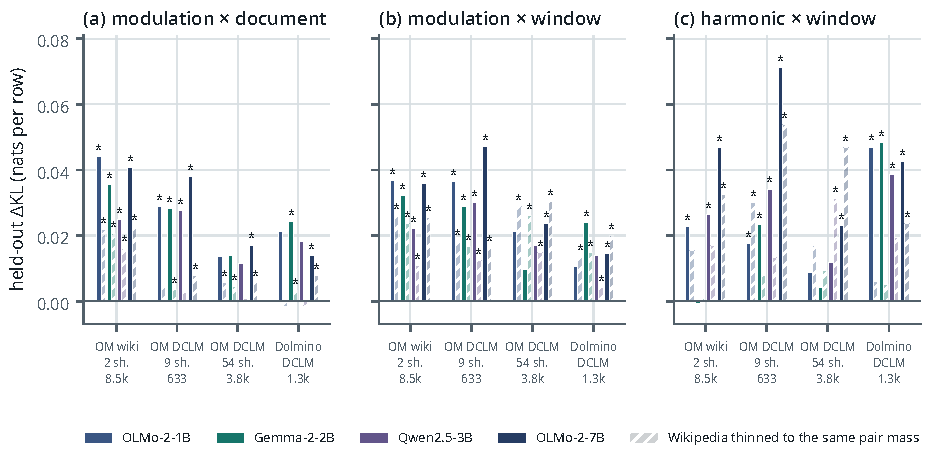
\includegraphics[width=.96\linewidth,keepaspectratio]{figures/fig_crosscorpus.pdf}
\kirinfigcaption{Figure C.1.}{Cross-corpus held-out gain (target-aggregated view). Panels show modulation$\times$document, modulation$\times$window and harmonic$\times$window. Solid: the corpus; hatched: Wikipedia thinned to the same number of pairs. The gain is present for every model from every corpus, sparse DCLM samples included; the sparsest real corpora beat thinned Wikipedia for OLMo and non-OLMo models alike, while at 3,843 pairs the window conditional falls below thinned Wikipedia for three of four models (panel b).}
\end{minipage}

DiD $=$ (OLMo models $-$ Gemma/Qwen) $\times$ (corpus $-$ size-matched Wikipedia); Wilcoxon over 15 source rows. The four cells displayed in the first draft are the harmonic and modulation rows of the window and document columns; the full set follows (target-aggregated view; spelled view in \texttt{results/phase5/crosscorpus\_compare\_spelled.txt}, \texttt{\_big\_spelled.txt}).
{\footnotesize
\begin{longtable}{@{}lcccc@{}}
\toprule
\kirintablehead{Corpus / family} & \hd{window} & \hd{cue} & \hd{document} \\
\midrule
\endhead
OLMo-Mix wiki, harmonic & $+0.007$ ($.01$) & $+0.015$ ($<.005$) & $+0.011$ ($.25$) \\
OLMo-Mix wiki, chord & $+0.007$ ($.09$) & $-0.000$ ($.64$) & $+0.025$ ($.39$) \\
OLMo-Mix wiki, modulation & $+0.001$ ($.45$) & $+0.007$ ($.39$) & $+0.008$ ($.04$) \\
OLMo-Mix DCLM (9 sh.), harmonic & $-0.016$ ($.21$) & $+0.021$ ($.36$) & $-0.006$ ($.76$) \\
OLMo-Mix DCLM (9 sh.), chord & $+0.012$ ($.52$) & $+0.023$ ($.15$) & $+0.018$ ($.17$) \\
OLMo-Mix DCLM (9 sh.), modulation & $+0.010$ ($.19$) & $-0.001$ ($.52$) & $+0.002$ ($.68$) \\
OLMo-Mix DCLM (54 sh.), harmonic & $-0.004$ ($.98$) & $-0.009$ ($.85$) & $-0.002$ ($.45$) \\
OLMo-Mix DCLM (54 sh.), chord & $-0.002$ ($.68$) & $-0.007$ ($.93$) & $+0.023$ ($.01$) \\
OLMo-Mix DCLM (54 sh.), modulation & $-0.000$ ($.76$) & $+0.000$ ($.76$) & $-0.000$ ($.85$) \\
Dolmino DCLM, harmonic & $-0.001$ ($.93$) & $+0.021$ ($.21$) & $-0.019$ ($.07$) \\
Dolmino DCLM, chord & $+0.020$ ($.19$) & $+0.001$ ($.80$) & $+0.049$ ($<.005$) \\
Dolmino DCLM, modulation & $-0.014$ ($.09$) & $-0.003$ ($.33$) & $-0.006$ ($.19$) \\
\bottomrule
\end{longtable}}
\noindent Spelled view, significant cells: OLMo-Mix wiki harmonic $\times$ window $+0.012$ ($.01$), harmonic $\times$ cue $+0.012$ ($.01$), modulation $\times$ document $+0.004$ ($.02$); 9-shard DCLM modulation $\times$ window $+0.005$ ($.01$); Dolmino chord $\times$ window $+0.017$ ($.02$); all nine cells of the 54-shard sample $p\ge.33$. The 54-shard sample was scanned after the other analyses (post-hoc expansion, declared in the log).

\subsection*{C.4 Synthetic factorial, final checkpoint (means over five seeds)}
\begin{longtable}{@{}lccccc@{}}
\toprule
\kirintablehead{Condition} & \hd{KL to oracle} & \hd{\cl} & \hd{\lc{} (oracle)} & \hd{twin-source JS} & \hd{twin-target asym.} \\
\midrule
\endhead
CIRCLE $\times$ aligned & $0.001$ & $0.976$ & $0.436$ ($0.439$) & $0.000$ & $0.101$ \\
CIRCLE $\times$ permuted & $0.001$ & $0.979$ & $0.422$ ($0.439$) & $0.000$ & $0.088$ \\
LINE $\times$ aligned & $0.000$ & $0.000$ & $0.995$ ($0.995$) & $0.564$ & $3.22$ \\
LINE $\times$ permuted & $0.001$ & $-0.008$ & $0.995$ ($0.995$) & $0.564$ & $3.23$ \\
\bottomrule
\end{longtable}
\noindent{\small The \cl{} column is the code-controlled partial; the \lc{} column is the uncontrolled partial, the one comparable across code conditions (\S\ref{sec:synthetic}); the code-controlled \lc{} values are $0.113$ / $0.421$ / $0.787$ / $0.995$.}

\subsection*{C.5 OLMo-2-1B checkpoints (modulation family)}
{\scriptsize
\begin{longtable}{@{}lcccc@{}}
\toprule
\kirintablehead{Checkpoint (tokens)} & \hd{\lc} & \hd{\cl} & \hd{residual, document ($p$)} & \hd{residual, window ($p$)} \\
\midrule
\endhead
stage 1, 1B & $-0.24$ & $+0.01$ & $+0.15$ ($.33$) & $-0.01$ ($.55$) \\
stage 1, 21B & $+0.19$ & $-0.09$ & $+0.14$ ($.51$) & $+0.10$ ($.49$) \\
stage 1, 49B & $+0.27$ & $-0.25$ & $+0.12$ ($.41$) & $+0.15$ ($.31$) \\
stage 1, 105B & $+0.27$ & $-0.09$ & $+0.27$ ($.10$) & $+0.23$ ($.10$) \\
stage 1, 294B & $+0.27$ & $-0.07$ & $+0.40$ ($.037$) & $+0.27$ ($.10$) \\
stage 1, 1007B & $+0.34$ & $-0.02$ & $+0.26$ ($.23$) & $+0.18$ ($.33$) \\
stage 1, 1993B & $+0.33$ & $-0.04$ & $+0.34$ ($.050$) & $+0.19$ ($.21$) \\
stage 1, 4001B & $+0.33$ & $-0.06$ & $+0.44$ ($.005$) & $+0.26$ ($.061$) \\
stage 2, seed 1 / 2 / 3 (51B) & $+0.42$ / $+0.42$ / $+0.44$ & $-0.03$ / $+0.02$ / $-0.01$ & $+0.48$ / $+0.45$ / $+0.46$ ($\le.017$) & $+0.28$ / $+0.27$ / $+0.27$ ($.06$--$.08$) \\
released model (other run) & $+0.47$ & $+0.03$ & $+0.53$ ($\le.0005$) & $+0.41$ ($.001$) \\
\bottomrule
\end{longtable}}



\subsection*{C.6 Scorer robustness of Result 3 (line$\,|\,$circle and circle$\,|\,$line, family means over four templates)}
Total sequence log-probability scorer vs the pre-registered length-normalized scorer; ``sig'' = templates with \lc{} significant under the glyph-preserving relabeling null ($B=1{,}000$, $b/B$); ECI = enharmonic collapse index of the behavioural matrix (total / length-normalized).
{\footnotesize
\begin{longtable}{@{}llccccccc@{}}
\toprule
\kirintablehead{Model} & \hd{Family} & \hd{total \lc} & \hd{total \cl} & \hd{sig} & \hd{norm.\ \lc} & \hd{norm.\ \cl} & \hd{sig} & \hd{ECI} \\
\midrule
\endhead
OLMo-2-1B & B enharmonic & $+0.30$ & $+0.07$ & 4/4 & $+0.28$ & $+0.08$ & 3/4 & 0.70/0.58 \\
OLMo-2-1B & C harmonic & $+0.33$ & $-0.03$ & 4/4 & $+0.21$ & $-0.00$ & 4/4 & 0.86/0.69 \\
OLMo-2-1B & D chord & $+0.27$ & $-0.10$ & 4/4 & $+0.19$ & $-0.06$ & 2/4 & 0.84/0.59 \\
OLMo-2-1B & E modulation & $+0.44$ & $+0.02$ & 4/4 & $+0.37$ & $+0.01$ & 4/4 & 0.88/0.81 \\
Gemma-2-2B & B enharmonic & $+0.50$ & $-0.14$ & 4/4 & $+0.45$ & $-0.07$ & 4/4 & 0.83/0.75 \\
Gemma-2-2B & C harmonic & $+0.32$ & $-0.00$ & 4/4 & $+0.24$ & $+0.03$ & 4/4 & 0.83/0.73 \\
Gemma-2-2B & D chord & $+0.36$ & $-0.14$ & 4/4 & $+0.26$ & $-0.03$ & 4/4 & 0.90/0.72 \\
Gemma-2-2B & E modulation & $+0.54$ & $-0.07$ & 4/4 & $+0.43$ & $+0.03$ & 4/4 & 0.90/0.85 \\
Qwen2.5-3B & B enharmonic & $+0.31$ & $+0.11$ & 4/4 & $+0.31$ & $+0.07$ & 4/4 & 0.51/0.38 \\
Qwen2.5-3B & C harmonic & $+0.42$ & $+0.11$ & 4/4 & $+0.27$ & $+0.09$ & 4/4 & 0.73/0.52 \\
Qwen2.5-3B & D chord & $+0.40$ & $-0.01$ & 4/4 & $+0.23$ & $+0.06$ & 3/4 & 0.78/0.57 \\
Qwen2.5-3B & E modulation & $+0.52$ & $+0.07$ & 4/4 & $+0.50$ & $+0.00$ & 4/4 & 0.88/0.79 \\
OLMo-2-7B & B enharmonic & $+0.14$ & $+0.28$ & 3/4 & $+0.19$ & $+0.25$ & 3/4 & 0.11/0.05 \\
OLMo-2-7B & C harmonic & $+0.38$ & $+0.16$ & 4/4 & $+0.38$ & $+0.09$ & 4/4 & 0.67/0.43 \\
OLMo-2-7B & D chord & $+0.50$ & $+0.13$ & 4/4 & $+0.38$ & $+0.16$ & 3/4 & 0.74/0.53 \\
OLMo-2-7B & E modulation & $+0.56$ & $+0.13$ & 4/4 & $+0.45$ & $+0.12$ & 4/4 & 0.81/0.68 \\
\bottomrule
\end{longtable}}

\subsection*{C.7 Template robustness of the flagship held-out gain}
Target-aggregated view, modulation family, $\Delta\KL$ (nats per row) for OLMo-1B / Gemma / Qwen / OLMo-7B when the behavioural matrix is built from a single template or from the leave-one-template-out mean; $^{\mathrm{ns}}$ marks relabeling $p\ge.05$ ($B=2{,}000$). Templates in the order of Appendix~D.4 (1: ``The piece modulates from \{x\} major to''; 2: ``The first movement is in \{x\} major and the second movement is in''; 3: ``The song, originally in \{x\} major, was later transposed to''; 4: ``The first song on the album is in \{x\} major. The second song is in'').
{\footnotesize
\begin{longtable}{@{}lll@{}}
\toprule
\kirintablehead{Templates} & \hd{window conditional} & \hd{document conditional} \\
\midrule
\endhead
template 1 only & $+0.058$ / $+0.035$ / $+0.018$ / $+0.041$ & $+0.066$ / $+0.047$ / $+0.019$ / $+0.043$ \\
template 2 only & $+0.044$ / $+0.028$ / $+0.023$ / $+0.043$ & $+0.052$ / $+0.043$ / $+0.032$ / $+0.059$ \\
template 3 only & $+0.018$ / $+0.022$ / $+0.007$$^{\mathrm{ns}}$ / $+0.008$$^{\mathrm{ns}}$ & $+0.030$ / $+0.016$ / $+0.016$$^{\mathrm{ns}}$ / $+0.004$$^{\mathrm{ns}}$ \\
template 4 only & $+0.026$ / $+0.030$ / $+0.020$ / $+0.051$ & $+0.030$ / $+0.036$ / $+0.030$ / $+0.051$ \\
all but 1 & $+0.028$ / $+0.027$ / $+0.016$ / $+0.033$ & $+0.036$ / $+0.032$ / $+0.025$ / $+0.038$ \\
all but 2 & $+0.034$ / $+0.030$ / $+0.015$ / $+0.033$ & $+0.043$ / $+0.034$ / $+0.020$ / $+0.032$ \\
all but 3 & $+0.044$ / $+0.031$ / $+0.020$ / $+0.046$ & $+0.050$ / $+0.042$ / $+0.027$ / $+0.052$ \\
all but 4 & $+0.041$ / $+0.029$ / $+0.016$ / $+0.030$ & $+0.051$ / $+0.036$ / $+0.022$ / $+0.035$ \\
\bottomrule
\end{longtable}}

\kirinpart{Appendix D}{Methods in full}

\subsection*{D.1 Keys, spellings and aliases}
The 12-key design uses the conventional spellings C, D\fl, D, E\fl, E, F, F\sh, G, A\fl, A, B\fl, B (semitone $x=0,\dots,11$; fifths position $7x \bmod 12$; signed accidental count $s=p$ for $p\le6$, $p-12$ otherwise). The 15-key design uses the standard major-key spellings on the signed line $s=-7,\dots,+7$: C\fl, G\fl, D\fl, A\fl, E\fl, B\fl, F, C, G, D, A, E, B, F\sh, C\sh; enharmonic pairs (C\fl, B), (G\fl, F\sh), (D\fl, C\sh). In text, symbol (C\#, Db), word (C-sharp, D flat, C sharp) and Unicode (C\sh, D\fl) forms are all mapped to the symbol spelling. In the merged 12-key family the two spellings of each pitch class are pooled (B\sh/C, D\fl/C\sh, E\fl/D\sh, F\fl/E, E\sh/F, G\fl/F\sh, A\fl/G\sh, B\fl/A\sh, C\fl/B) before counting.

\subsection*{D.2 Corpus matching and symmetric statistics}
Corpus: the \texttt{wikimedia/wikipedia} \texttt{20231101.en} parquet release (41 shards, 6.41M documents, $\approx3.1$B whitespace-delimited words). A key mention is a match of the pattern \texttt{[A-G](accidental)?\textvisiblespace(major|minor)}, not preceded by an alphanumeric character or hyphen and not followed by a letter; matches at sentence-initial position (preceded, ignoring spaces, by a sentence-final or opening character, or at document start) are excluded from unigram and pair counts because ``A major'' is ambiguous there. Symmetric statistics follow \citet{karkada2026symmetry}: for every ordered token pair within a window of $L=16$ words the pair count is incremented by $f(d)=17-d$ with $d$ the word distance; $Z$ is the $f$-weighted number of (position, offset) pairs and $N$ the number of word tokens; $\rho_{ij}=(C_{ij}/Z)/((n_i/N)(n_j/N))$; $M^*=2(\rho-1)/(\rho+1)$ and $\mathrm{PMI}=\log\rho$, with zero-count cells floored one unit below the minimum observed PMI. Group tallies (all documents, documents mentioning ``circle of fifths''/``perfect fifth'', and the rest) are kept separately.

\subsection*{D.3 Conditional (ordered key-mention) statistics}
For each document containing `` major'', the major-key mentions are listed in order with their character offsets (15 spellings only). Family A: for each ordered pair of mentions $(a,b)$ with $b$ after $a$, if the segment between the end of $a$ and the start of $b$ contains at most 40 whitespace-delimited words, $N^{A}_{k(a),k(b)}$ is incremented by one (all such pairs, including repeated mentions; the scan stops at the first later mention beyond 40 words). Family B increments $N^{B_c}$ for the same pairs when the intervening segment contains a cue from class $c$ (modulation, chord, key-signature, enharmonic, relation; \texttt{phase5/scan\_conditional.py} lists the cue strings); B\_any is the union. Family C matches four relational regular expressions. Family D increments $N^{D}_{k,k'}$ once per document for every pair of keys whose first mentions occur in that order. The corpus predictor is $\log C_{ij}=\log\frac{N_{ij}+0.5}{\sum_{j'}(N_{ij'}+0.5)}$ over the 15 target spellings; in the target-aggregated view the columns are merged by log-sum-exp over each pitch class. Per-document count matrices are stored for the cluster bootstrap.

\subsection*{D.4 Behavioural scoring}
For a template $t$ of family $f$ and source key $x_i$, the prompt is $t$ with \{x\} replaced by the symbol spelling of $x_i$ (e.g.\ ``The piece modulates from D\fl{} major to''). Each of the 15 candidates is the string ``\textvisiblespace$x_j$\textvisiblespace major'' appended to the prompt and tokenized without special tokens; the model's log-softmax over the vocabulary is evaluated once on the concatenated sequence (teacher forcing) and the candidate score is the sum of the log-probabilities of the candidate's tokens at their positions. The \emph{total} scorer uses this sum, the \emph{length-normalized} scorer divides it by the candidate's token count, and the \emph{enharmonic-merged behavioural scorer} log-sum-exps the two spellings of each twin before normalizing (applied to families B, C, D only). Scores are log-softmax-normalized over the 15 candidates within a row; the family matrix used in \S\ref{sec:heldout} is the mean over the family's four templates of the per-template row-normalized log-probabilities, renormalized. Precision: OLMo-2-1B and its checkpoints in fp32; Gemma-2-2B, Qwen2.5-3B and OLMo-2-7B in bf16 (a bf16/fp32 check on OLMo-2-1B changed Fourier shares by $\le0.002$). Prompt templates:
\begin{longtable}{@{}lp{0.80\linewidth}@{}}
\toprule
\kirintablehead{Family} & \hd{Templates (\{x\} = source key)} \\
\midrule
\endhead
A spelling & The key signature of \{x\} major has $\cdot$ In \{x\} major, the accidentals written in the key signature are $\cdot$ Spelled correctly, the scale of \{x\} major uses the notes $\cdot$ The number of sharps or flats in the key signature of \{x\} major is \\
B enharmonic & On the piano, the tonic of \{x\} major is the same key as the tonic of $\cdot$ In equal temperament, \{x\} major sounds identical to $\cdot$ The enharmonic equivalent of \{x\} major is $\cdot$ Played on a keyboard, a piece in \{x\} major uses the same keys as a piece in \\
C harmonic & The dominant key of \{x\} major is $\cdot$ The subdominant key of \{x\} major is $\cdot$ A key closely related to \{x\} major is $\cdot$ The relative minor of \{x\} major shares its key signature with \\
D chord & In the key of \{x\} major, the tonic chord is usually followed by the chord of $\cdot$ A typical chord progression in \{x\} major moves from the tonic chord to the chord of $\cdot$ In \{x\} major, the perfect cadence resolves from the dominant chord to the chord of $\cdot$ Improvising over a song in \{x\} major, the guitarist played the chord of \\
E modulation & The piece modulates from \{x\} major to $\cdot$ The first movement is in \{x\} major and the second movement is in $\cdot$ The song, originally in \{x\} major, was later transposed to $\cdot$ The first song on the album is in \{x\} major. The second song is in \\
F generic & She said the piece was in \{x\} major and everyone $\cdot$ The recording of the sonata in \{x\} major was released in $\cdot$ Most listeners preferred the version in \{x\} major because $\cdot$ The manuscript of the symphony in \{x\} major is kept in \\
\bottomrule
\end{longtable}

\subsection*{D.5 Models and hidden-state positions}
\texttt{allenai/OLMo-2-0425-1B} (revision \texttt{main} as of 2026-08-28; checkpoint branches \texttt{stage1-step300-tokens1B}, \texttt{-step10000-tokens21B}, \texttt{-step23100-tokens49B}, \texttt{-step50000-tokens105B}, \texttt{-step140000-tokens294B}, \texttt{-step480000-tokens1007B}, \texttt{-step950000-tokens1993B}, \texttt{-step1907359-tokens4001B}, \texttt{stage2-ingredient\{1,2,3\}-step23852-tokens51B}); \texttt{unsloth/gemma-2-2b} (a bf16 safetensors mirror of \texttt{google/gemma-2-2b}, used because the original repository is gated); \texttt{Qwen/Qwen2.5-3B}; \texttt{allenai/OLMo-2-1124-7B}. Hidden states are taken at every layer at three positions: the last token of the key name (the accidental token for two-token spellings), the mean over the key-name span, and the prompt-final token; token counts of each spelling under each tokenizer enter the theory features. Layer bands for context contrasts are the middle half of the network, fixed before the results.

\subsection*{D.6 The held-out regression of \S\ref{sec:heldout}}
\emph{Response.} $y_{ij}=\log Q_{ij}$, the family-mean row-normalized log-probability of target $j$ given source $i$, over all ordered off-diagonal pairs (210 in the spelled view; 165 in the target-aggregated view, where $j$ ranges over the 11 classes other than the source's own). \emph{Corpus predictor.} $c_{ij}=\log C_{ij}$ as in D.3 (a single column). \emph{Theory features.} Spelled view: circle distance, line distance, signed difference $s_j-s_i$, glyph-class equality, has-accidental($i$), has-accidental($j$), same root letter, Levenshtein distance of the spellings, $\log(n_i+1)$, $\log(n_j+1)$, token count($i$), token count($j$); target-aggregated view: circle distance, line distance to the class's mean line position, signed difference, has-accidental($i$), $\log(n_i+1)$, log class frequency, token count($i$). The \emph{rich} model adds the squares of the three distances, circle$\times$line, and $\cos(2\pi k\,d_c/12)$ for $k=1,2,3$. The \emph{target-prior} control (\S\ref{sec:heldout}) adds, for each held-out row, the mean of $y_{\cdot j}$ over the 14 training rows as a feature (recomputed inside every fold; the held-out row is never used). Features are z-scored over all pairs (a scaling that uses the held-out row's feature values but not its response). \emph{Estimator.} Ridge regression with an unpenalized intercept and penalty $\lambda=1$ on the standardized coefficients, fixed a priori and not tuned; predictors: theory features only, corpus column only, theory + corpus. \emph{Hold-out.} For each source $i$, fit on the pairs of the other 14 rows and predict the held-out row's targets; the predicted log-scores are log-softmax-normalized over the held-out row's targets, and $\mathrm{KL}(q_i\,\|\,\hat q_i)$ is computed with the actual row $q_i$ renormalized over the same targets ($10^{-12}$ added inside the log); $\Delta\mathrm{KL}$ is the mean over the 15 rows of KL(theory) $-$ KL(theory + corpus); the within-row $R^2$ gain is $1-\mathrm{SSE}_{\text{both}}/\mathrm{SSE}_{\text{theory}}$ with rows centred; $\Delta$CV is the mean within-row Spearman difference. \emph{Nulls.} The corpus count matrix's rows and columns are permuted jointly by a random relabeling of the 15 keys (the model matrix and features fixed), the whole procedure is recomputed, and $p=(b+1)/(B+1)$ with $b$ the number of null statistics at least as large as the observed one; $B=5{,}000$ for the Wikipedia analyses, $2{,}000$ for the cross-corpus and checkpoint analyses, $500$ for the Phase-II geometry nulls and $1{,}000$ for the Phase-II behaviour nulls (the latter two computed as $b/B$; adding one to numerator and denominator changes them by at most $0.002$). \emph{Bootstraps.} Corpus sampling uncertainty of the flagship $\Delta\mathrm{KL}$ is from a document-cluster bootstrap (the 9,168 key-mentioning documents resampled with replacement, count matrices and frequency features rebuilt, 300 resamples); Phase-I corpus statistics use the shard-cluster bootstrap of Result~1. Residual correspondence (\S\ref{sec:heldout}, test 1) regresses $y$ and $c$ on the same features over all pairs and reports the Spearman correlation of the residuals with the same relabeling null.

\end{document}
